\documentclass[twoside]{book}

% Packages required by doxygen
\usepackage{fixltx2e}
\usepackage{calc}
\usepackage{doxygen}
\usepackage[export]{adjustbox} % also loads graphicx
\usepackage{graphicx}
\usepackage[utf8]{inputenc}
\usepackage{makeidx}
\usepackage{multicol}
\usepackage{multirow}
\PassOptionsToPackage{warn}{textcomp}
\usepackage{textcomp}
\usepackage[nointegrals]{wasysym}
\usepackage[table]{xcolor}

% Font selection
\usepackage[T1]{fontenc}
\usepackage[scaled=.90]{helvet}
\usepackage{courier}
\usepackage{amssymb}
\usepackage{sectsty}
\renewcommand{\familydefault}{\sfdefault}
\allsectionsfont{%
  \fontseries{bc}\selectfont%
  \color{darkgray}%
}
\renewcommand{\DoxyLabelFont}{%
  \fontseries{bc}\selectfont%
  \color{darkgray}%
}
\newcommand{\+}{\discretionary{\mbox{\scriptsize$\hookleftarrow$}}{}{}}

% Page & text layout
\usepackage{geometry}
\geometry{%
  a4paper,%
  top=2.5cm,%
  bottom=2.5cm,%
  left=2.5cm,%
  right=2.5cm%
}
\tolerance=750
\hfuzz=15pt
\hbadness=750
\setlength{\emergencystretch}{15pt}
\setlength{\parindent}{0cm}
\setlength{\parskip}{3ex plus 2ex minus 2ex}
\makeatletter
\renewcommand{\paragraph}{%
  \@startsection{paragraph}{4}{0ex}{-1.0ex}{1.0ex}{%
    \normalfont\normalsize\bfseries\SS@parafont%
  }%
}
\renewcommand{\subparagraph}{%
  \@startsection{subparagraph}{5}{0ex}{-1.0ex}{1.0ex}{%
    \normalfont\normalsize\bfseries\SS@subparafont%
  }%
}
\makeatother

% Headers & footers
\usepackage{fancyhdr}
\pagestyle{fancyplain}
\fancyhead[LE]{\fancyplain{}{\bfseries\thepage}}
\fancyhead[CE]{\fancyplain{}{}}
\fancyhead[RE]{\fancyplain{}{\bfseries\leftmark}}
\fancyhead[LO]{\fancyplain{}{\bfseries\rightmark}}
\fancyhead[CO]{\fancyplain{}{}}
\fancyhead[RO]{\fancyplain{}{\bfseries\thepage}}
\fancyfoot[LE]{\fancyplain{}{}}
\fancyfoot[CE]{\fancyplain{}{}}
\fancyfoot[RE]{\fancyplain{}{\bfseries\scriptsize Generated by Doxygen }}
\fancyfoot[LO]{\fancyplain{}{\bfseries\scriptsize Generated by Doxygen }}
\fancyfoot[CO]{\fancyplain{}{}}
\fancyfoot[RO]{\fancyplain{}{}}
\renewcommand{\footrulewidth}{0.4pt}
\renewcommand{\chaptermark}[1]{%
  \markboth{#1}{}%
}
\renewcommand{\sectionmark}[1]{%
  \markright{\thesection\ #1}%
}

% Indices & bibliography
\usepackage{natbib}
\usepackage[titles]{tocloft}
\setcounter{tocdepth}{3}
\setcounter{secnumdepth}{5}
\makeindex

% Hyperlinks (required, but should be loaded last)
\usepackage{ifpdf}
\ifpdf
  \usepackage[pdftex,pagebackref=true]{hyperref}
\else
  \usepackage[ps2pdf,pagebackref=true]{hyperref}
\fi
\hypersetup{%
  colorlinks=true,%
  linkcolor=blue,%
  citecolor=blue,%
  unicode%
}

% Custom commands
\newcommand{\clearemptydoublepage}{%
  \newpage{\pagestyle{empty}\cleardoublepage}%
}

\usepackage{caption}
\captionsetup{labelsep=space,justification=centering,font={bf},singlelinecheck=off,skip=4pt,position=top}

%===== C O N T E N T S =====

\begin{document}

% Titlepage & ToC
\hypersetup{pageanchor=false,
             bookmarksnumbered=true,
             pdfencoding=unicode
            }
\pagenumbering{alph}
\begin{titlepage}
\vspace*{7cm}
\begin{center}%
{\Large Snake Battle Royale (S\+BR) \\[1ex]\large 1.\+0 }\\
\vspace*{1cm}
{\large Generated by Doxygen 1.8.14}\\
\end{center}
\end{titlepage}
\clearemptydoublepage
\pagenumbering{roman}
\tableofcontents
\clearemptydoublepage
\pagenumbering{arabic}
\hypersetup{pageanchor=true}

%--- Begin generated contents ---
\chapter{Namespace Index}
\section{Packages}
Here are the packages with brief descriptions (if available)\+:\begin{DoxyCompactList}
\item\contentsline{section}{\mbox{\hyperlink{namespacesnakegame}{snakegame}} }{\pageref{namespacesnakegame}}{}
\item\contentsline{section}{\mbox{\hyperlink{namespacesnakegame_1_1client}{snakegame.\+client}} }{\pageref{namespacesnakegame_1_1client}}{}
\item\contentsline{section}{\mbox{\hyperlink{namespacesnakegame_1_1server}{snakegame.\+server}} }{\pageref{namespacesnakegame_1_1server}}{}
\item\contentsline{section}{\mbox{\hyperlink{namespacesnakegame_1_1structs}{snakegame.\+structs}} }{\pageref{namespacesnakegame_1_1structs}}{}
\end{DoxyCompactList}

\chapter{Hierarchical Index}
\section{Class Hierarchy}
This inheritance list is sorted roughly, but not completely, alphabetically\+:\begin{DoxyCompactList}
\item \contentsline{section}{snakegame.\+structs.\+Apple}{\pageref{classsnakegame_1_1structs_1_1_apple}}{}
\item \contentsline{section}{snakegame.\+structs.\+Apple\+Factory}{\pageref{classsnakegame_1_1structs_1_1_apple_factory}}{}
\item \contentsline{section}{snakegame.\+server.\+Server.\+Client\+Updater}{\pageref{classsnakegame_1_1server_1_1_server_1_1_client_updater}}{}
\item Cloneable\begin{DoxyCompactList}
\item \contentsline{section}{snakegame.\+structs.\+Remainder}{\pageref{classsnakegame_1_1structs_1_1_remainder}}{}
\end{DoxyCompactList}
\item \contentsline{section}{snakegame.\+Constants}{\pageref{classsnakegame_1_1_constants}}{}
\begin{DoxyCompactList}
\item \contentsline{section}{snakegame.\+apple}{\pageref{classsnakegame_1_1apple}}{}
\item \contentsline{section}{snakegame.\+snake}{\pageref{classsnakegame_1_1snake}}{}
\end{DoxyCompactList}
\item \contentsline{section}{snakegame.\+server.\+Contriols\+Queue}{\pageref{classsnakegame_1_1server_1_1_contriols_queue}}{}
\item \contentsline{section}{snakegame.\+structs.\+Direction}{\pageref{enumsnakegame_1_1structs_1_1_direction}}{}
\item \contentsline{section}{snakegame.\+Game}{\pageref{classsnakegame_1_1_game}}{}
\item J\+Frame\begin{DoxyCompactList}
\item \contentsline{section}{snakegame.\+client.\+Client}{\pageref{classsnakegame_1_1client_1_1_client}}{}
\item \contentsline{section}{snakegame.\+Main\+Window}{\pageref{classsnakegame_1_1_main_window}}{}
\end{DoxyCompactList}
\item \contentsline{section}{snakegame.\+server.\+Message}{\pageref{classsnakegame_1_1server_1_1_message}}{}
\item \contentsline{section}{snakegame.\+structs.\+Point}{\pageref{classsnakegame_1_1structs_1_1_point}}{}
\begin{DoxyCompactList}
\item \contentsline{section}{snakegame.\+structs.\+Apple\+Point}{\pageref{classsnakegame_1_1structs_1_1_apple_point}}{}
\item \contentsline{section}{snakegame.\+structs.\+Snake\+Point}{\pageref{classsnakegame_1_1structs_1_1_snake_point}}{}
\end{DoxyCompactList}
\item Runnable\begin{DoxyCompactList}
\item \contentsline{section}{snakegame.\+server.\+Server.\+Client\+Handler}{\pageref{classsnakegame_1_1server_1_1_server_1_1_client_handler}}{}
\item \contentsline{section}{snakegame.\+server.\+Server.\+World\+Updater}{\pageref{classsnakegame_1_1server_1_1_server_1_1_world_updater}}{}
\end{DoxyCompactList}
\item \contentsline{section}{snakegame.\+server.\+Server}{\pageref{classsnakegame_1_1server_1_1_server}}{}
\item \contentsline{section}{snakegame.\+structs.\+Snake}{\pageref{classsnakegame_1_1structs_1_1_snake}}{}
\item \contentsline{section}{snakegame.\+structs.\+Snake\+Factory}{\pageref{classsnakegame_1_1structs_1_1_snake_factory}}{}
\item \contentsline{section}{snakegame.\+structs.\+World}{\pageref{classsnakegame_1_1structs_1_1_world}}{}
\end{DoxyCompactList}

\chapter{Class Index}
\section{Class List}
Here are the classes, structs, unions and interfaces with brief descriptions\+:\begin{DoxyCompactList}
\item\contentsline{section}{\mbox{\hyperlink{classsnakegame_1_1apple}{snakegame.\+apple}} }{\pageref{classsnakegame_1_1apple}}{}
\item\contentsline{section}{\mbox{\hyperlink{classsnakegame_1_1structs_1_1_apple}{snakegame.\+structs.\+Apple}} }{\pageref{classsnakegame_1_1structs_1_1_apple}}{}
\item\contentsline{section}{\mbox{\hyperlink{classsnakegame_1_1structs_1_1_apple_factory}{snakegame.\+structs.\+Apple\+Factory}} }{\pageref{classsnakegame_1_1structs_1_1_apple_factory}}{}
\item\contentsline{section}{\mbox{\hyperlink{classsnakegame_1_1structs_1_1_apple_point}{snakegame.\+structs.\+Apple\+Point}} }{\pageref{classsnakegame_1_1structs_1_1_apple_point}}{}
\item\contentsline{section}{\mbox{\hyperlink{classsnakegame_1_1client_1_1_client}{snakegame.\+client.\+Client}} }{\pageref{classsnakegame_1_1client_1_1_client}}{}
\item\contentsline{section}{\mbox{\hyperlink{classsnakegame_1_1server_1_1_server_1_1_client_handler}{snakegame.\+server.\+Server.\+Client\+Handler}} }{\pageref{classsnakegame_1_1server_1_1_server_1_1_client_handler}}{}
\item\contentsline{section}{\mbox{\hyperlink{classsnakegame_1_1server_1_1_server_1_1_client_updater}{snakegame.\+server.\+Server.\+Client\+Updater}} }{\pageref{classsnakegame_1_1server_1_1_server_1_1_client_updater}}{}
\item\contentsline{section}{\mbox{\hyperlink{classsnakegame_1_1_constants}{snakegame.\+Constants}} }{\pageref{classsnakegame_1_1_constants}}{}
\item\contentsline{section}{\mbox{\hyperlink{classsnakegame_1_1server_1_1_contriols_queue}{snakegame.\+server.\+Contriols\+Queue}} }{\pageref{classsnakegame_1_1server_1_1_contriols_queue}}{}
\item\contentsline{section}{\mbox{\hyperlink{enumsnakegame_1_1structs_1_1_direction}{snakegame.\+structs.\+Direction}} }{\pageref{enumsnakegame_1_1structs_1_1_direction}}{}
\item\contentsline{section}{\mbox{\hyperlink{classsnakegame_1_1_game}{snakegame.\+Game}} }{\pageref{classsnakegame_1_1_game}}{}
\item\contentsline{section}{\mbox{\hyperlink{classsnakegame_1_1_main_window}{snakegame.\+Main\+Window}} }{\pageref{classsnakegame_1_1_main_window}}{}
\item\contentsline{section}{\mbox{\hyperlink{classsnakegame_1_1server_1_1_message}{snakegame.\+server.\+Message}} }{\pageref{classsnakegame_1_1server_1_1_message}}{}
\item\contentsline{section}{\mbox{\hyperlink{classsnakegame_1_1structs_1_1_point}{snakegame.\+structs.\+Point}} }{\pageref{classsnakegame_1_1structs_1_1_point}}{}
\item\contentsline{section}{\mbox{\hyperlink{classsnakegame_1_1structs_1_1_remainder}{snakegame.\+structs.\+Remainder}} }{\pageref{classsnakegame_1_1structs_1_1_remainder}}{}
\item\contentsline{section}{\mbox{\hyperlink{classsnakegame_1_1server_1_1_server}{snakegame.\+server.\+Server}} }{\pageref{classsnakegame_1_1server_1_1_server}}{}
\item\contentsline{section}{\mbox{\hyperlink{classsnakegame_1_1structs_1_1_snake}{snakegame.\+structs.\+Snake}} }{\pageref{classsnakegame_1_1structs_1_1_snake}}{}
\item\contentsline{section}{\mbox{\hyperlink{classsnakegame_1_1snake}{snakegame.\+snake}} }{\pageref{classsnakegame_1_1snake}}{}
\item\contentsline{section}{\mbox{\hyperlink{classsnakegame_1_1structs_1_1_snake_factory}{snakegame.\+structs.\+Snake\+Factory}} }{\pageref{classsnakegame_1_1structs_1_1_snake_factory}}{}
\item\contentsline{section}{\mbox{\hyperlink{classsnakegame_1_1structs_1_1_snake_point}{snakegame.\+structs.\+Snake\+Point}} }{\pageref{classsnakegame_1_1structs_1_1_snake_point}}{}
\item\contentsline{section}{\mbox{\hyperlink{classsnakegame_1_1structs_1_1_world}{snakegame.\+structs.\+World}} }{\pageref{classsnakegame_1_1structs_1_1_world}}{}
\item\contentsline{section}{\mbox{\hyperlink{classsnakegame_1_1server_1_1_server_1_1_world_updater}{snakegame.\+server.\+Server.\+World\+Updater}} }{\pageref{classsnakegame_1_1server_1_1_server_1_1_world_updater}}{}
\end{DoxyCompactList}

\chapter{File Index}
\section{File List}
Here is a list of all files with brief descriptions\+:\begin{DoxyCompactList}
\item\contentsline{section}{src/snakegame/\mbox{\hyperlink{apple_8java}{apple.\+java}} }{\pageref{apple_8java}}{}
\item\contentsline{section}{src/snakegame/\mbox{\hyperlink{_constants_8java}{Constants.\+java}} }{\pageref{_constants_8java}}{}
\item\contentsline{section}{src/snakegame/\mbox{\hyperlink{_game_8java}{Game.\+java}} }{\pageref{_game_8java}}{}
\item\contentsline{section}{src/snakegame/\mbox{\hyperlink{_main_window_8java}{Main\+Window.\+java}} }{\pageref{_main_window_8java}}{}
\item\contentsline{section}{src/snakegame/\mbox{\hyperlink{snake_8java}{snake.\+java}} }{\pageref{snake_8java}}{}
\item\contentsline{section}{src/snakegame/client/\mbox{\hyperlink{_client_8java}{Client.\+java}} }{\pageref{_client_8java}}{}
\item\contentsline{section}{src/snakegame/server/\mbox{\hyperlink{_contriols_queue_8java}{Contriols\+Queue.\+java}} }{\pageref{_contriols_queue_8java}}{}
\item\contentsline{section}{src/snakegame/server/\mbox{\hyperlink{_message_8java}{Message.\+java}} }{\pageref{_message_8java}}{}
\item\contentsline{section}{src/snakegame/server/\mbox{\hyperlink{_server_8java}{Server.\+java}} }{\pageref{_server_8java}}{}
\item\contentsline{section}{src/snakegame/structs/\mbox{\hyperlink{structs_2apple_8java}{Apple.\+java}} }{\pageref{structs_2apple_8java}}{}
\item\contentsline{section}{src/snakegame/structs/\mbox{\hyperlink{_apple_factory_8java}{Apple\+Factory.\+java}} }{\pageref{_apple_factory_8java}}{}
\item\contentsline{section}{src/snakegame/structs/\mbox{\hyperlink{_apple_point_8java}{Apple\+Point.\+java}} }{\pageref{_apple_point_8java}}{}
\item\contentsline{section}{src/snakegame/structs/\mbox{\hyperlink{_direction_8java}{Direction.\+java}} }{\pageref{_direction_8java}}{}
\item\contentsline{section}{src/snakegame/structs/\mbox{\hyperlink{_point_8java}{Point.\+java}} }{\pageref{_point_8java}}{}
\item\contentsline{section}{src/snakegame/structs/\mbox{\hyperlink{_remainder_8java}{Remainder.\+java}} }{\pageref{_remainder_8java}}{}
\item\contentsline{section}{src/snakegame/structs/\mbox{\hyperlink{structs_2snake_8java}{Snake.\+java}} }{\pageref{structs_2snake_8java}}{}
\item\contentsline{section}{src/snakegame/structs/\mbox{\hyperlink{_snake_factory_8java}{Snake\+Factory.\+java}} }{\pageref{_snake_factory_8java}}{}
\item\contentsline{section}{src/snakegame/structs/\mbox{\hyperlink{_snake_point_8java}{Snake\+Point.\+java}} }{\pageref{_snake_point_8java}}{}
\item\contentsline{section}{src/snakegame/structs/\mbox{\hyperlink{_world_8java}{World.\+java}} }{\pageref{_world_8java}}{}
\end{DoxyCompactList}

\chapter{Namespace Documentation}
\hypertarget{namespacesnakegame}{}\section{Package snakegame}
\label{namespacesnakegame}\index{snakegame@{snakegame}}
\subsection*{Packages}
\begin{DoxyCompactItemize}
\item 
package \mbox{\hyperlink{namespacesnakegame_1_1client}{client}}
\item 
package \mbox{\hyperlink{namespacesnakegame_1_1server}{server}}
\item 
package \mbox{\hyperlink{namespacesnakegame_1_1structs}{structs}}
\end{DoxyCompactItemize}
\subsection*{Classes}
\begin{DoxyCompactItemize}
\item 
class \mbox{\hyperlink{classsnakegame_1_1apple}{apple}}
\item 
class \mbox{\hyperlink{classsnakegame_1_1_constants}{Constants}}
\item 
class \mbox{\hyperlink{classsnakegame_1_1_game}{Game}}
\item 
class \mbox{\hyperlink{classsnakegame_1_1_main_window}{Main\+Window}}
\item 
class \mbox{\hyperlink{classsnakegame_1_1snake}{snake}}
\end{DoxyCompactItemize}

\hypertarget{namespacesnakegame_1_1client}{}\section{Package snakegame.\+client}
\label{namespacesnakegame_1_1client}\index{snakegame.\+client@{snakegame.\+client}}
\subsection*{Classes}
\begin{DoxyCompactItemize}
\item 
class \mbox{\hyperlink{classsnakegame_1_1client_1_1_client}{Client}}
\end{DoxyCompactItemize}

\hypertarget{namespacesnakegame_1_1server}{}\section{Package snakegame.\+server}
\label{namespacesnakegame_1_1server}\index{snakegame.\+server@{snakegame.\+server}}
\subsection*{Classes}
\begin{DoxyCompactItemize}
\item 
class \mbox{\hyperlink{classsnakegame_1_1server_1_1_contriols_queue}{Contriols\+Queue}}
\item 
class \mbox{\hyperlink{classsnakegame_1_1server_1_1_message}{Message}}
\item 
class \mbox{\hyperlink{classsnakegame_1_1server_1_1_server}{Server}}
\end{DoxyCompactItemize}

\hypertarget{namespacesnakegame_1_1structs}{}\section{Package snakegame.\+structs}
\label{namespacesnakegame_1_1structs}\index{snakegame.\+structs@{snakegame.\+structs}}
\subsection*{Classes}
\begin{DoxyCompactItemize}
\item 
class \mbox{\hyperlink{classsnakegame_1_1structs_1_1_apple}{Apple}}
\item 
class \mbox{\hyperlink{classsnakegame_1_1structs_1_1_apple_factory}{Apple\+Factory}}
\item 
class \mbox{\hyperlink{classsnakegame_1_1structs_1_1_apple_point}{Apple\+Point}}
\item 
enum \mbox{\hyperlink{enumsnakegame_1_1structs_1_1_direction}{Direction}}
\item 
class \mbox{\hyperlink{classsnakegame_1_1structs_1_1_point}{Point}}
\item 
class \mbox{\hyperlink{classsnakegame_1_1structs_1_1_remainder}{Remainder}}
\item 
class \mbox{\hyperlink{classsnakegame_1_1structs_1_1_snake}{Snake}}
\item 
class \mbox{\hyperlink{classsnakegame_1_1structs_1_1_snake_factory}{Snake\+Factory}}
\item 
class \mbox{\hyperlink{classsnakegame_1_1structs_1_1_snake_point}{Snake\+Point}}
\item 
class \mbox{\hyperlink{classsnakegame_1_1structs_1_1_world}{World}}
\end{DoxyCompactItemize}

\chapter{Class Documentation}
\hypertarget{classsnakegame_1_1apple}{}\section{snakegame.\+apple Class Reference}
\label{classsnakegame_1_1apple}\index{snakegame.\+apple@{snakegame.\+apple}}
Inheritance diagram for snakegame.\+apple\+:\begin{figure}[H]
\begin{center}
\leavevmode
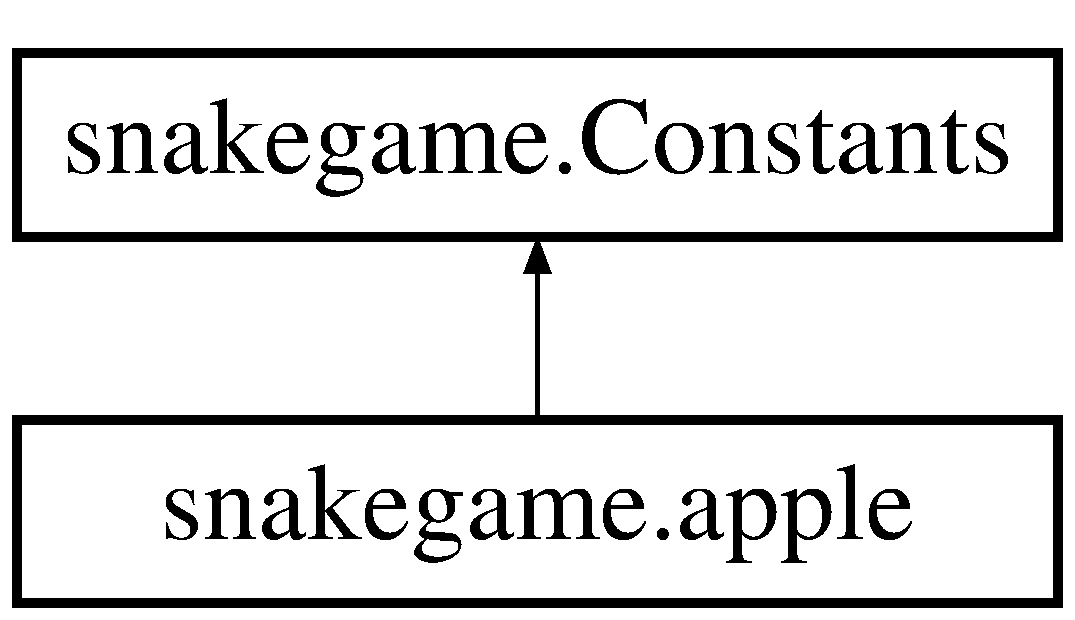
\includegraphics[height=2.000000cm]{classsnakegame_1_1apple}
\end{center}
\end{figure}
\subsection*{Public Member Functions}
\begin{DoxyCompactItemize}
\item 
Point \mbox{\hyperlink{classsnakegame_1_1apple_a2a93c78385af6c64271ce163dd883712}{apple1}} ()
\item 
void \mbox{\hyperlink{classsnakegame_1_1apple_af5cab740833aef8650ef374868585930}{set}} ()
\item 
void \mbox{\hyperlink{classsnakegame_1_1apple_a4868669a889a955b0811141726005a23}{set}} (boolean a)
\item 
void \mbox{\hyperlink{classsnakegame_1_1apple_aa14da591e5ca8e5ce41da4ace3dfd8af}{set}} (\mbox{\hyperlink{classsnakegame_1_1apple}{apple}} ap2)
\item 
void \mbox{\hyperlink{classsnakegame_1_1apple_a3a6294f277af9a64dea186eb41583b97}{paint}} (Graphics2D g2)
\end{DoxyCompactItemize}
\subsection*{Additional Inherited Members}


\subsection{Detailed Description}


Definition at line 6 of file apple.\+java.



\subsection{Member Function Documentation}
\mbox{\Hypertarget{classsnakegame_1_1apple_a2a93c78385af6c64271ce163dd883712}\label{classsnakegame_1_1apple_a2a93c78385af6c64271ce163dd883712}} 
\index{snakegame\+::apple@{snakegame\+::apple}!apple1@{apple1}}
\index{apple1@{apple1}!snakegame\+::apple@{snakegame\+::apple}}
\subsubsection{\texorpdfstring{apple1()}{apple1()}}
{\footnotesize\ttfamily Point snakegame.\+apple.\+apple1 (\begin{DoxyParamCaption}{ }\end{DoxyParamCaption})}



Definition at line 23 of file apple.\+java.

\mbox{\Hypertarget{classsnakegame_1_1apple_a3a6294f277af9a64dea186eb41583b97}\label{classsnakegame_1_1apple_a3a6294f277af9a64dea186eb41583b97}} 
\index{snakegame\+::apple@{snakegame\+::apple}!paint@{paint}}
\index{paint@{paint}!snakegame\+::apple@{snakegame\+::apple}}
\subsubsection{\texorpdfstring{paint()}{paint()}}
{\footnotesize\ttfamily void snakegame.\+apple.\+paint (\begin{DoxyParamCaption}\item[{Graphics2D}]{g2 }\end{DoxyParamCaption})}



Definition at line 43 of file apple.\+java.

\mbox{\Hypertarget{classsnakegame_1_1apple_af5cab740833aef8650ef374868585930}\label{classsnakegame_1_1apple_af5cab740833aef8650ef374868585930}} 
\index{snakegame\+::apple@{snakegame\+::apple}!set@{set}}
\index{set@{set}!snakegame\+::apple@{snakegame\+::apple}}
\subsubsection{\texorpdfstring{set()}{set()}\hspace{0.1cm}{\footnotesize\ttfamily [1/3]}}
{\footnotesize\ttfamily void snakegame.\+apple.\+set (\begin{DoxyParamCaption}{ }\end{DoxyParamCaption})}



Definition at line 24 of file apple.\+java.

\mbox{\Hypertarget{classsnakegame_1_1apple_a4868669a889a955b0811141726005a23}\label{classsnakegame_1_1apple_a4868669a889a955b0811141726005a23}} 
\index{snakegame\+::apple@{snakegame\+::apple}!set@{set}}
\index{set@{set}!snakegame\+::apple@{snakegame\+::apple}}
\subsubsection{\texorpdfstring{set()}{set()}\hspace{0.1cm}{\footnotesize\ttfamily [2/3]}}
{\footnotesize\ttfamily void snakegame.\+apple.\+set (\begin{DoxyParamCaption}\item[{boolean}]{a }\end{DoxyParamCaption})}



Definition at line 32 of file apple.\+java.

\mbox{\Hypertarget{classsnakegame_1_1apple_aa14da591e5ca8e5ce41da4ace3dfd8af}\label{classsnakegame_1_1apple_aa14da591e5ca8e5ce41da4ace3dfd8af}} 
\index{snakegame\+::apple@{snakegame\+::apple}!set@{set}}
\index{set@{set}!snakegame\+::apple@{snakegame\+::apple}}
\subsubsection{\texorpdfstring{set()}{set()}\hspace{0.1cm}{\footnotesize\ttfamily [3/3]}}
{\footnotesize\ttfamily void snakegame.\+apple.\+set (\begin{DoxyParamCaption}\item[{\mbox{\hyperlink{classsnakegame_1_1apple}{apple}}}]{ap2 }\end{DoxyParamCaption})}



Definition at line 36 of file apple.\+java.



The documentation for this class was generated from the following file\+:\begin{DoxyCompactItemize}
\item 
src/snakegame/\mbox{\hyperlink{apple_8java}{apple.\+java}}\end{DoxyCompactItemize}

\hypertarget{classsnakegame_1_1structs_1_1_apple}{}\section{snakegame.\+structs.\+Apple Class Reference}
\label{classsnakegame_1_1structs_1_1_apple}\index{snakegame.\+structs.\+Apple@{snakegame.\+structs.\+Apple}}
\subsection*{Public Member Functions}
\begin{DoxyCompactItemize}
\item 
\mbox{\hyperlink{classsnakegame_1_1structs_1_1_apple_a396350cfc8fdecede585381c93150a6d}{Apple}} (\mbox{\hyperlink{classsnakegame_1_1structs_1_1_apple_point}{Apple\+Point}} point)
\item 
\mbox{\hyperlink{classsnakegame_1_1structs_1_1_apple_point}{Apple\+Point}} \mbox{\hyperlink{classsnakegame_1_1structs_1_1_apple_a1c6cf6198f99833004b657097596fd64}{get\+Point}} ()
\item 
void \mbox{\hyperlink{classsnakegame_1_1structs_1_1_apple_ae92b2f9ad12f097c9bfa5f408270f8f2}{draw}} (Graphics2D g)
\item 
String \mbox{\hyperlink{classsnakegame_1_1structs_1_1_apple_abebdf6e508f4ce621f460cd95d498028}{to\+String}} ()
\end{DoxyCompactItemize}
\subsection*{Static Public Member Functions}
\begin{DoxyCompactItemize}
\item 
static \mbox{\hyperlink{classsnakegame_1_1structs_1_1_apple}{Apple}} \mbox{\hyperlink{classsnakegame_1_1structs_1_1_apple_aa7282ddcff4a6529e95e679a2a57ec5b}{parse}} (String string)
\end{DoxyCompactItemize}


\subsection{Detailed Description}


Definition at line 6 of file Apple.\+java.



\subsection{Constructor \& Destructor Documentation}
\mbox{\Hypertarget{classsnakegame_1_1structs_1_1_apple_a396350cfc8fdecede585381c93150a6d}\label{classsnakegame_1_1structs_1_1_apple_a396350cfc8fdecede585381c93150a6d}} 
\index{snakegame\+::structs\+::\+Apple@{snakegame\+::structs\+::\+Apple}!Apple@{Apple}}
\index{Apple@{Apple}!snakegame\+::structs\+::\+Apple@{snakegame\+::structs\+::\+Apple}}
\subsubsection{\texorpdfstring{Apple()}{Apple()}}
{\footnotesize\ttfamily snakegame.\+structs.\+Apple.\+Apple (\begin{DoxyParamCaption}\item[{\mbox{\hyperlink{classsnakegame_1_1structs_1_1_apple_point}{Apple\+Point}}}]{point }\end{DoxyParamCaption})}



Definition at line 8 of file Apple.\+java.



\subsection{Member Function Documentation}
\mbox{\Hypertarget{classsnakegame_1_1structs_1_1_apple_ae92b2f9ad12f097c9bfa5f408270f8f2}\label{classsnakegame_1_1structs_1_1_apple_ae92b2f9ad12f097c9bfa5f408270f8f2}} 
\index{snakegame\+::structs\+::\+Apple@{snakegame\+::structs\+::\+Apple}!draw@{draw}}
\index{draw@{draw}!snakegame\+::structs\+::\+Apple@{snakegame\+::structs\+::\+Apple}}
\subsubsection{\texorpdfstring{draw()}{draw()}}
{\footnotesize\ttfamily void snakegame.\+structs.\+Apple.\+draw (\begin{DoxyParamCaption}\item[{Graphics2D}]{g }\end{DoxyParamCaption})}



Definition at line 18 of file Apple.\+java.

\mbox{\Hypertarget{classsnakegame_1_1structs_1_1_apple_a1c6cf6198f99833004b657097596fd64}\label{classsnakegame_1_1structs_1_1_apple_a1c6cf6198f99833004b657097596fd64}} 
\index{snakegame\+::structs\+::\+Apple@{snakegame\+::structs\+::\+Apple}!get\+Point@{get\+Point}}
\index{get\+Point@{get\+Point}!snakegame\+::structs\+::\+Apple@{snakegame\+::structs\+::\+Apple}}
\subsubsection{\texorpdfstring{get\+Point()}{getPoint()}}
{\footnotesize\ttfamily \mbox{\hyperlink{classsnakegame_1_1structs_1_1_apple_point}{Apple\+Point}} snakegame.\+structs.\+Apple.\+get\+Point (\begin{DoxyParamCaption}{ }\end{DoxyParamCaption})}



Definition at line 14 of file Apple.\+java.

\mbox{\Hypertarget{classsnakegame_1_1structs_1_1_apple_aa7282ddcff4a6529e95e679a2a57ec5b}\label{classsnakegame_1_1structs_1_1_apple_aa7282ddcff4a6529e95e679a2a57ec5b}} 
\index{snakegame\+::structs\+::\+Apple@{snakegame\+::structs\+::\+Apple}!parse@{parse}}
\index{parse@{parse}!snakegame\+::structs\+::\+Apple@{snakegame\+::structs\+::\+Apple}}
\subsubsection{\texorpdfstring{parse()}{parse()}}
{\footnotesize\ttfamily static \mbox{\hyperlink{classsnakegame_1_1structs_1_1_apple}{Apple}} snakegame.\+structs.\+Apple.\+parse (\begin{DoxyParamCaption}\item[{String}]{string }\end{DoxyParamCaption})\hspace{0.3cm}{\ttfamily [static]}}



Definition at line 34 of file Apple.\+java.

\mbox{\Hypertarget{classsnakegame_1_1structs_1_1_apple_abebdf6e508f4ce621f460cd95d498028}\label{classsnakegame_1_1structs_1_1_apple_abebdf6e508f4ce621f460cd95d498028}} 
\index{snakegame\+::structs\+::\+Apple@{snakegame\+::structs\+::\+Apple}!to\+String@{to\+String}}
\index{to\+String@{to\+String}!snakegame\+::structs\+::\+Apple@{snakegame\+::structs\+::\+Apple}}
\subsubsection{\texorpdfstring{to\+String()}{toString()}}
{\footnotesize\ttfamily String snakegame.\+structs.\+Apple.\+to\+String (\begin{DoxyParamCaption}{ }\end{DoxyParamCaption})}



Definition at line 23 of file Apple.\+java.



The documentation for this class was generated from the following file\+:\begin{DoxyCompactItemize}
\item 
src/snakegame/structs/\mbox{\hyperlink{structs_2apple_8java}{Apple.\+java}}\end{DoxyCompactItemize}

\hypertarget{classsnakegame_1_1structs_1_1_apple_factory}{}\section{snakegame.\+structs.\+Apple\+Factory Class Reference}
\label{classsnakegame_1_1structs_1_1_apple_factory}\index{snakegame.\+structs.\+Apple\+Factory@{snakegame.\+structs.\+Apple\+Factory}}
\subsection*{Public Member Functions}
\begin{DoxyCompactItemize}
\item 
\mbox{\hyperlink{classsnakegame_1_1structs_1_1_apple_factory_ac58956184a77beb43d78d6f1a72b3254}{Apple\+Factory}} (List$<$ \mbox{\hyperlink{classsnakegame_1_1structs_1_1_apple_point}{Apple\+Point}} $>$ points)
\item 
\mbox{\hyperlink{classsnakegame_1_1structs_1_1_apple_factory_acc49c3b4cda4250fd4a25181b39cb36e}{Apple\+Factory}} ()
\item 
\mbox{\hyperlink{classsnakegame_1_1structs_1_1_apple}{Apple}} \mbox{\hyperlink{classsnakegame_1_1structs_1_1_apple_factory_a53efb1530e63916af192eb4daa0009f6}{generate\+Apple}} ()
\end{DoxyCompactItemize}


\subsection{Detailed Description}


Definition at line 8 of file Apple\+Factory.\+java.



\subsection{Constructor \& Destructor Documentation}
\mbox{\Hypertarget{classsnakegame_1_1structs_1_1_apple_factory_ac58956184a77beb43d78d6f1a72b3254}\label{classsnakegame_1_1structs_1_1_apple_factory_ac58956184a77beb43d78d6f1a72b3254}} 
\index{snakegame\+::structs\+::\+Apple\+Factory@{snakegame\+::structs\+::\+Apple\+Factory}!Apple\+Factory@{Apple\+Factory}}
\index{Apple\+Factory@{Apple\+Factory}!snakegame\+::structs\+::\+Apple\+Factory@{snakegame\+::structs\+::\+Apple\+Factory}}
\subsubsection{\texorpdfstring{Apple\+Factory()}{AppleFactory()}\hspace{0.1cm}{\footnotesize\ttfamily [1/2]}}
{\footnotesize\ttfamily snakegame.\+structs.\+Apple\+Factory.\+Apple\+Factory (\begin{DoxyParamCaption}\item[{List$<$ \mbox{\hyperlink{classsnakegame_1_1structs_1_1_apple_point}{Apple\+Point}} $>$}]{points }\end{DoxyParamCaption})}



Definition at line 17 of file Apple\+Factory.\+java.

\mbox{\Hypertarget{classsnakegame_1_1structs_1_1_apple_factory_acc49c3b4cda4250fd4a25181b39cb36e}\label{classsnakegame_1_1structs_1_1_apple_factory_acc49c3b4cda4250fd4a25181b39cb36e}} 
\index{snakegame\+::structs\+::\+Apple\+Factory@{snakegame\+::structs\+::\+Apple\+Factory}!Apple\+Factory@{Apple\+Factory}}
\index{Apple\+Factory@{Apple\+Factory}!snakegame\+::structs\+::\+Apple\+Factory@{snakegame\+::structs\+::\+Apple\+Factory}}
\subsubsection{\texorpdfstring{Apple\+Factory()}{AppleFactory()}\hspace{0.1cm}{\footnotesize\ttfamily [2/2]}}
{\footnotesize\ttfamily snakegame.\+structs.\+Apple\+Factory.\+Apple\+Factory (\begin{DoxyParamCaption}{ }\end{DoxyParamCaption})}



Definition at line 25 of file Apple\+Factory.\+java.



\subsection{Member Function Documentation}
\mbox{\Hypertarget{classsnakegame_1_1structs_1_1_apple_factory_a53efb1530e63916af192eb4daa0009f6}\label{classsnakegame_1_1structs_1_1_apple_factory_a53efb1530e63916af192eb4daa0009f6}} 
\index{snakegame\+::structs\+::\+Apple\+Factory@{snakegame\+::structs\+::\+Apple\+Factory}!generate\+Apple@{generate\+Apple}}
\index{generate\+Apple@{generate\+Apple}!snakegame\+::structs\+::\+Apple\+Factory@{snakegame\+::structs\+::\+Apple\+Factory}}
\subsubsection{\texorpdfstring{generate\+Apple()}{generateApple()}}
{\footnotesize\ttfamily \mbox{\hyperlink{classsnakegame_1_1structs_1_1_apple}{Apple}} snakegame.\+structs.\+Apple\+Factory.\+generate\+Apple (\begin{DoxyParamCaption}{ }\end{DoxyParamCaption})}



Definition at line 36 of file Apple\+Factory.\+java.



The documentation for this class was generated from the following file\+:\begin{DoxyCompactItemize}
\item 
src/snakegame/structs/\mbox{\hyperlink{_apple_factory_8java}{Apple\+Factory.\+java}}\end{DoxyCompactItemize}

\hypertarget{classsnakegame_1_1structs_1_1_apple_point}{}\section{snakegame.\+structs.\+Apple\+Point Class Reference}
\label{classsnakegame_1_1structs_1_1_apple_point}\index{snakegame.\+structs.\+Apple\+Point@{snakegame.\+structs.\+Apple\+Point}}
Inheritance diagram for snakegame.\+structs.\+Apple\+Point\+:\begin{figure}[H]
\begin{center}
\leavevmode
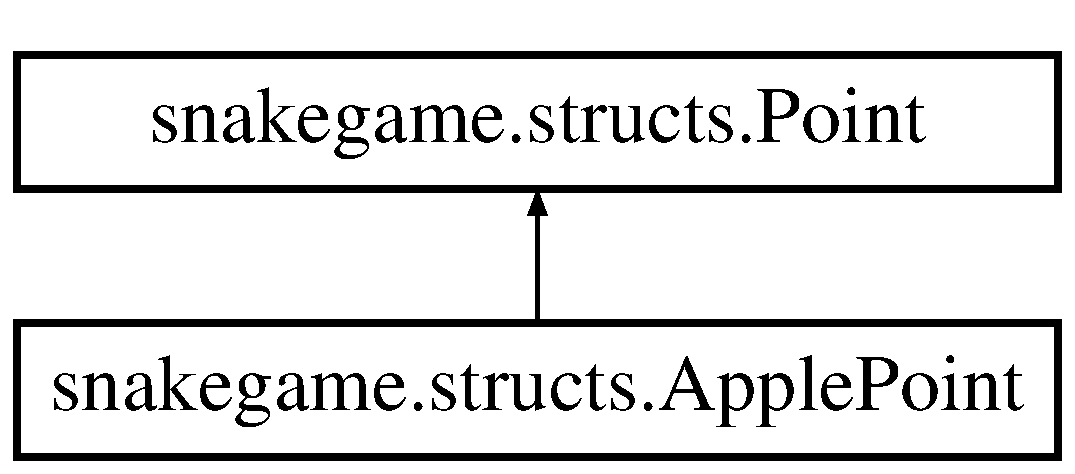
\includegraphics[height=2.000000cm]{classsnakegame_1_1structs_1_1_apple_point}
\end{center}
\end{figure}
\subsection*{Public Member Functions}
\begin{DoxyCompactItemize}
\item 
\mbox{\hyperlink{classsnakegame_1_1structs_1_1_apple_point_a4d23b0796de73346c556ee8e10bcf080}{Apple\+Point}} (\mbox{\hyperlink{classsnakegame_1_1structs_1_1_remainder}{Remainder}} \mbox{\hyperlink{classsnakegame_1_1structs_1_1_point_acf6c91ee7cda0e65a8054ff0dc07b79a}{x}}, \mbox{\hyperlink{classsnakegame_1_1structs_1_1_remainder}{Remainder}} \mbox{\hyperlink{classsnakegame_1_1structs_1_1_point_a2a9fe55d9cf57dbc120bbce39313d38d}{y}})
\item 
void \mbox{\hyperlink{classsnakegame_1_1structs_1_1_apple_point_a0202e1a32a56ad9778cea65a604282c6}{draw}} (Graphics2D g)
\end{DoxyCompactItemize}
\subsection*{Additional Inherited Members}


\subsection{Detailed Description}


Definition at line 5 of file Apple\+Point.\+java.



\subsection{Constructor \& Destructor Documentation}
\mbox{\Hypertarget{classsnakegame_1_1structs_1_1_apple_point_a4d23b0796de73346c556ee8e10bcf080}\label{classsnakegame_1_1structs_1_1_apple_point_a4d23b0796de73346c556ee8e10bcf080}} 
\index{snakegame\+::structs\+::\+Apple\+Point@{snakegame\+::structs\+::\+Apple\+Point}!Apple\+Point@{Apple\+Point}}
\index{Apple\+Point@{Apple\+Point}!snakegame\+::structs\+::\+Apple\+Point@{snakegame\+::structs\+::\+Apple\+Point}}
\subsubsection{\texorpdfstring{Apple\+Point()}{ApplePoint()}}
{\footnotesize\ttfamily snakegame.\+structs.\+Apple\+Point.\+Apple\+Point (\begin{DoxyParamCaption}\item[{\mbox{\hyperlink{classsnakegame_1_1structs_1_1_remainder}{Remainder}}}]{x,  }\item[{\mbox{\hyperlink{classsnakegame_1_1structs_1_1_remainder}{Remainder}}}]{y }\end{DoxyParamCaption})}



Definition at line 8 of file Apple\+Point.\+java.



\subsection{Member Function Documentation}
\mbox{\Hypertarget{classsnakegame_1_1structs_1_1_apple_point_a0202e1a32a56ad9778cea65a604282c6}\label{classsnakegame_1_1structs_1_1_apple_point_a0202e1a32a56ad9778cea65a604282c6}} 
\index{snakegame\+::structs\+::\+Apple\+Point@{snakegame\+::structs\+::\+Apple\+Point}!draw@{draw}}
\index{draw@{draw}!snakegame\+::structs\+::\+Apple\+Point@{snakegame\+::structs\+::\+Apple\+Point}}
\subsubsection{\texorpdfstring{draw()}{draw()}}
{\footnotesize\ttfamily void snakegame.\+structs.\+Apple\+Point.\+draw (\begin{DoxyParamCaption}\item[{Graphics2D}]{g }\end{DoxyParamCaption})}



Definition at line 14 of file Apple\+Point.\+java.



The documentation for this class was generated from the following file\+:\begin{DoxyCompactItemize}
\item 
src/snakegame/structs/\mbox{\hyperlink{_apple_point_8java}{Apple\+Point.\+java}}\end{DoxyCompactItemize}

\hypertarget{classsnakegame_1_1client_1_1_client}{}\section{snakegame.\+client.\+Client Class Reference}
\label{classsnakegame_1_1client_1_1_client}\index{snakegame.\+client.\+Client@{snakegame.\+client.\+Client}}
Inheritance diagram for snakegame.\+client.\+Client\+:\begin{figure}[H]
\begin{center}
\leavevmode
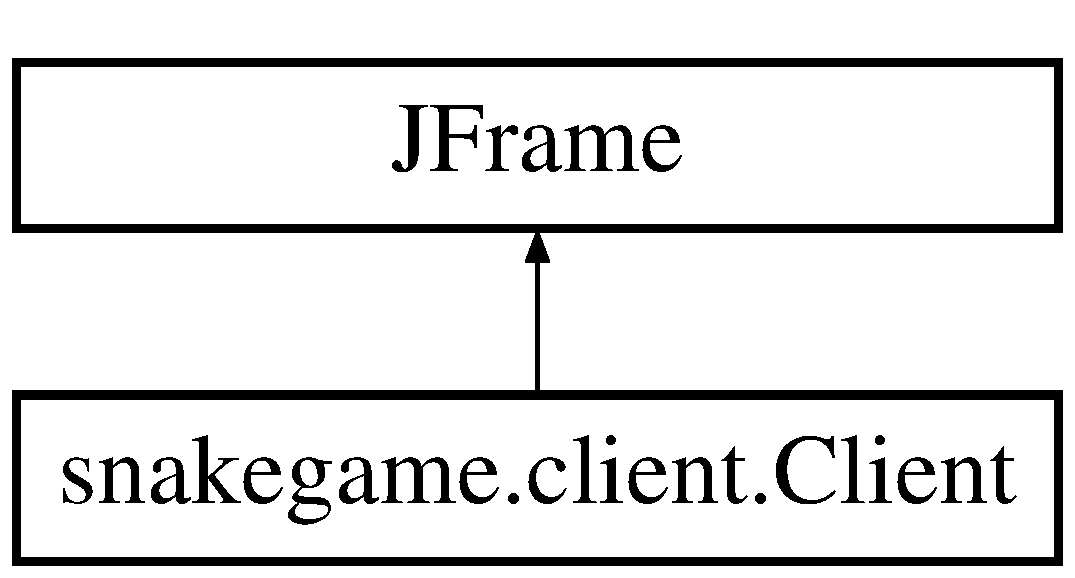
\includegraphics[height=2.000000cm]{classsnakegame_1_1client_1_1_client}
\end{center}
\end{figure}
\subsection*{Classes}
\begin{DoxyCompactItemize}
\item 
class {\bfseries Client\+Key\+Listener}
\end{DoxyCompactItemize}
\subsection*{Public Member Functions}
\begin{DoxyCompactItemize}
\item 
\mbox{\hyperlink{classsnakegame_1_1client_1_1_client_a1d9ca3c932bb8594efdfc6facb33d90c}{Client}} (int port, String host)
\item 
\mbox{\hyperlink{classsnakegame_1_1client_1_1_client_a535018f1c145ab1ea9949f231b39bd42}{Client}} ()
\item 
\mbox{\hyperlink{classsnakegame_1_1client_1_1_client_a4165aaf5d9c01f9b4b9416ea5a60c84d}{Client}} (int port)
\item 
\mbox{\hyperlink{classsnakegame_1_1client_1_1_client_ac6777539a79418c36d55da33dc3451c5}{Client}} (String host)
\item 
void \mbox{\hyperlink{classsnakegame_1_1client_1_1_client_a4c8965e3e5776858c2c44bfba1fc0554}{run}} ()  throws I\+O\+Exception 
\item 
void \mbox{\hyperlink{classsnakegame_1_1client_1_1_client_a1e984a95002244e56d80be35396bf80e}{paint}} (Graphics g)
\end{DoxyCompactItemize}
\subsection*{Static Public Member Functions}
\begin{DoxyCompactItemize}
\item 
static void \mbox{\hyperlink{classsnakegame_1_1client_1_1_client_a0ff707341d32324b30dbb72b4ca90083}{main}} (String\mbox{[}$\,$\mbox{]} args)
\end{DoxyCompactItemize}


\subsection{Detailed Description}


Definition at line 24 of file Client.\+java.



\subsection{Constructor \& Destructor Documentation}
\mbox{\Hypertarget{classsnakegame_1_1client_1_1_client_a1d9ca3c932bb8594efdfc6facb33d90c}\label{classsnakegame_1_1client_1_1_client_a1d9ca3c932bb8594efdfc6facb33d90c}} 
\index{snakegame\+::client\+::\+Client@{snakegame\+::client\+::\+Client}!Client@{Client}}
\index{Client@{Client}!snakegame\+::client\+::\+Client@{snakegame\+::client\+::\+Client}}
\subsubsection{\texorpdfstring{Client()}{Client()}\hspace{0.1cm}{\footnotesize\ttfamily [1/4]}}
{\footnotesize\ttfamily snakegame.\+client.\+Client.\+Client (\begin{DoxyParamCaption}\item[{int}]{port,  }\item[{String}]{host }\end{DoxyParamCaption})}



Definition at line 35 of file Client.\+java.

\mbox{\Hypertarget{classsnakegame_1_1client_1_1_client_a535018f1c145ab1ea9949f231b39bd42}\label{classsnakegame_1_1client_1_1_client_a535018f1c145ab1ea9949f231b39bd42}} 
\index{snakegame\+::client\+::\+Client@{snakegame\+::client\+::\+Client}!Client@{Client}}
\index{Client@{Client}!snakegame\+::client\+::\+Client@{snakegame\+::client\+::\+Client}}
\subsubsection{\texorpdfstring{Client()}{Client()}\hspace{0.1cm}{\footnotesize\ttfamily [2/4]}}
{\footnotesize\ttfamily snakegame.\+client.\+Client.\+Client (\begin{DoxyParamCaption}{ }\end{DoxyParamCaption})}



Definition at line 71 of file Client.\+java.

\mbox{\Hypertarget{classsnakegame_1_1client_1_1_client_a4165aaf5d9c01f9b4b9416ea5a60c84d}\label{classsnakegame_1_1client_1_1_client_a4165aaf5d9c01f9b4b9416ea5a60c84d}} 
\index{snakegame\+::client\+::\+Client@{snakegame\+::client\+::\+Client}!Client@{Client}}
\index{Client@{Client}!snakegame\+::client\+::\+Client@{snakegame\+::client\+::\+Client}}
\subsubsection{\texorpdfstring{Client()}{Client()}\hspace{0.1cm}{\footnotesize\ttfamily [3/4]}}
{\footnotesize\ttfamily snakegame.\+client.\+Client.\+Client (\begin{DoxyParamCaption}\item[{int}]{port }\end{DoxyParamCaption})}



Definition at line 75 of file Client.\+java.

\mbox{\Hypertarget{classsnakegame_1_1client_1_1_client_ac6777539a79418c36d55da33dc3451c5}\label{classsnakegame_1_1client_1_1_client_ac6777539a79418c36d55da33dc3451c5}} 
\index{snakegame\+::client\+::\+Client@{snakegame\+::client\+::\+Client}!Client@{Client}}
\index{Client@{Client}!snakegame\+::client\+::\+Client@{snakegame\+::client\+::\+Client}}
\subsubsection{\texorpdfstring{Client()}{Client()}\hspace{0.1cm}{\footnotesize\ttfamily [4/4]}}
{\footnotesize\ttfamily snakegame.\+client.\+Client.\+Client (\begin{DoxyParamCaption}\item[{String}]{host }\end{DoxyParamCaption})}



Definition at line 77 of file Client.\+java.



\subsection{Member Function Documentation}
\mbox{\Hypertarget{classsnakegame_1_1client_1_1_client_a0ff707341d32324b30dbb72b4ca90083}\label{classsnakegame_1_1client_1_1_client_a0ff707341d32324b30dbb72b4ca90083}} 
\index{snakegame\+::client\+::\+Client@{snakegame\+::client\+::\+Client}!main@{main}}
\index{main@{main}!snakegame\+::client\+::\+Client@{snakegame\+::client\+::\+Client}}
\subsubsection{\texorpdfstring{main()}{main()}}
{\footnotesize\ttfamily static void snakegame.\+client.\+Client.\+main (\begin{DoxyParamCaption}\item[{String \mbox{[}$\,$\mbox{]}}]{args }\end{DoxyParamCaption})\hspace{0.3cm}{\ttfamily [static]}}



Definition at line 98 of file Client.\+java.

\mbox{\Hypertarget{classsnakegame_1_1client_1_1_client_a1e984a95002244e56d80be35396bf80e}\label{classsnakegame_1_1client_1_1_client_a1e984a95002244e56d80be35396bf80e}} 
\index{snakegame\+::client\+::\+Client@{snakegame\+::client\+::\+Client}!paint@{paint}}
\index{paint@{paint}!snakegame\+::client\+::\+Client@{snakegame\+::client\+::\+Client}}
\subsubsection{\texorpdfstring{paint()}{paint()}}
{\footnotesize\ttfamily void snakegame.\+client.\+Client.\+paint (\begin{DoxyParamCaption}\item[{Graphics}]{g }\end{DoxyParamCaption})}



Definition at line 107 of file Client.\+java.

\mbox{\Hypertarget{classsnakegame_1_1client_1_1_client_a4c8965e3e5776858c2c44bfba1fc0554}\label{classsnakegame_1_1client_1_1_client_a4c8965e3e5776858c2c44bfba1fc0554}} 
\index{snakegame\+::client\+::\+Client@{snakegame\+::client\+::\+Client}!run@{run}}
\index{run@{run}!snakegame\+::client\+::\+Client@{snakegame\+::client\+::\+Client}}
\subsubsection{\texorpdfstring{run()}{run()}}
{\footnotesize\ttfamily void snakegame.\+client.\+Client.\+run (\begin{DoxyParamCaption}{ }\end{DoxyParamCaption}) throws I\+O\+Exception}



Definition at line 80 of file Client.\+java.



The documentation for this class was generated from the following file\+:\begin{DoxyCompactItemize}
\item 
src/snakegame/client/\mbox{\hyperlink{_client_8java}{Client.\+java}}\end{DoxyCompactItemize}

\hypertarget{classsnakegame_1_1server_1_1_server_1_1_client_handler}{}\section{snakegame.\+server.\+Server.\+Client\+Handler Class Reference}
\label{classsnakegame_1_1server_1_1_server_1_1_client_handler}\index{snakegame.\+server.\+Server.\+Client\+Handler@{snakegame.\+server.\+Server.\+Client\+Handler}}
Inheritance diagram for snakegame.\+server.\+Server.\+Client\+Handler\+:\begin{figure}[H]
\begin{center}
\leavevmode
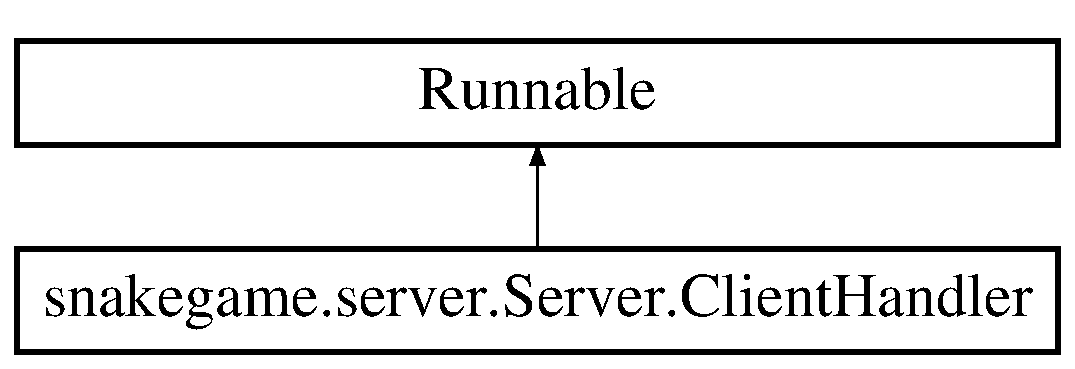
\includegraphics[height=2.000000cm]{classsnakegame_1_1server_1_1_server_1_1_client_handler}
\end{center}
\end{figure}
\subsection*{Public Member Functions}
\begin{DoxyCompactItemize}
\item 
\mbox{\hyperlink{classsnakegame_1_1server_1_1_server_1_1_client_handler_ad00a7d1d8e8ee23d5495fbe27d734828}{Client\+Handler}} (Socket socket)
\item 
void \mbox{\hyperlink{classsnakegame_1_1server_1_1_server_1_1_client_handler_a5cb1108121c65a4e73e8c55e0f6d97e8}{run}} ()
\end{DoxyCompactItemize}


\subsection{Detailed Description}


Definition at line 82 of file Server.\+java.



\subsection{Constructor \& Destructor Documentation}
\mbox{\Hypertarget{classsnakegame_1_1server_1_1_server_1_1_client_handler_ad00a7d1d8e8ee23d5495fbe27d734828}\label{classsnakegame_1_1server_1_1_server_1_1_client_handler_ad00a7d1d8e8ee23d5495fbe27d734828}} 
\index{snakegame\+::server\+::\+Server\+::\+Client\+Handler@{snakegame\+::server\+::\+Server\+::\+Client\+Handler}!Client\+Handler@{Client\+Handler}}
\index{Client\+Handler@{Client\+Handler}!snakegame\+::server\+::\+Server\+::\+Client\+Handler@{snakegame\+::server\+::\+Server\+::\+Client\+Handler}}
\subsubsection{\texorpdfstring{Client\+Handler()}{ClientHandler()}}
{\footnotesize\ttfamily snakegame.\+server.\+Server.\+Client\+Handler.\+Client\+Handler (\begin{DoxyParamCaption}\item[{Socket}]{socket }\end{DoxyParamCaption})}



Definition at line 88 of file Server.\+java.



\subsection{Member Function Documentation}
\mbox{\Hypertarget{classsnakegame_1_1server_1_1_server_1_1_client_handler_a5cb1108121c65a4e73e8c55e0f6d97e8}\label{classsnakegame_1_1server_1_1_server_1_1_client_handler_a5cb1108121c65a4e73e8c55e0f6d97e8}} 
\index{snakegame\+::server\+::\+Server\+::\+Client\+Handler@{snakegame\+::server\+::\+Server\+::\+Client\+Handler}!run@{run}}
\index{run@{run}!snakegame\+::server\+::\+Server\+::\+Client\+Handler@{snakegame\+::server\+::\+Server\+::\+Client\+Handler}}
\subsubsection{\texorpdfstring{run()}{run()}}
{\footnotesize\ttfamily void snakegame.\+server.\+Server.\+Client\+Handler.\+run (\begin{DoxyParamCaption}{ }\end{DoxyParamCaption})}



Definition at line 100 of file Server.\+java.



The documentation for this class was generated from the following file\+:\begin{DoxyCompactItemize}
\item 
src/snakegame/server/\mbox{\hyperlink{_server_8java}{Server.\+java}}\end{DoxyCompactItemize}

\hypertarget{classsnakegame_1_1server_1_1_server_1_1_client_updater}{}\section{snakegame.\+server.\+Server.\+Client\+Updater Class Reference}
\label{classsnakegame_1_1server_1_1_server_1_1_client_updater}\index{snakegame.\+server.\+Server.\+Client\+Updater@{snakegame.\+server.\+Server.\+Client\+Updater}}
\subsection*{Public Member Functions}
\begin{DoxyCompactItemize}
\item 
\mbox{\hyperlink{classsnakegame_1_1server_1_1_server_1_1_client_updater_a7cb2b186e3342d82f6e9b587ae5d22a4}{Client\+Updater}} (Socket socket)
\item 
void \mbox{\hyperlink{classsnakegame_1_1server_1_1_server_1_1_client_updater_a6a2031e0b0fdd55cf7d5c0eeb0b1e267}{publish}} ()  throws I\+O\+Exception 
\end{DoxyCompactItemize}


\subsection{Detailed Description}


Definition at line 137 of file Server.\+java.



\subsection{Constructor \& Destructor Documentation}
\mbox{\Hypertarget{classsnakegame_1_1server_1_1_server_1_1_client_updater_a7cb2b186e3342d82f6e9b587ae5d22a4}\label{classsnakegame_1_1server_1_1_server_1_1_client_updater_a7cb2b186e3342d82f6e9b587ae5d22a4}} 
\index{snakegame\+::server\+::\+Server\+::\+Client\+Updater@{snakegame\+::server\+::\+Server\+::\+Client\+Updater}!Client\+Updater@{Client\+Updater}}
\index{Client\+Updater@{Client\+Updater}!snakegame\+::server\+::\+Server\+::\+Client\+Updater@{snakegame\+::server\+::\+Server\+::\+Client\+Updater}}
\subsubsection{\texorpdfstring{Client\+Updater()}{ClientUpdater()}}
{\footnotesize\ttfamily snakegame.\+server.\+Server.\+Client\+Updater.\+Client\+Updater (\begin{DoxyParamCaption}\item[{Socket}]{socket }\end{DoxyParamCaption})}



Definition at line 141 of file Server.\+java.



\subsection{Member Function Documentation}
\mbox{\Hypertarget{classsnakegame_1_1server_1_1_server_1_1_client_updater_a6a2031e0b0fdd55cf7d5c0eeb0b1e267}\label{classsnakegame_1_1server_1_1_server_1_1_client_updater_a6a2031e0b0fdd55cf7d5c0eeb0b1e267}} 
\index{snakegame\+::server\+::\+Server\+::\+Client\+Updater@{snakegame\+::server\+::\+Server\+::\+Client\+Updater}!publish@{publish}}
\index{publish@{publish}!snakegame\+::server\+::\+Server\+::\+Client\+Updater@{snakegame\+::server\+::\+Server\+::\+Client\+Updater}}
\subsubsection{\texorpdfstring{publish()}{publish()}}
{\footnotesize\ttfamily void snakegame.\+server.\+Server.\+Client\+Updater.\+publish (\begin{DoxyParamCaption}{ }\end{DoxyParamCaption}) throws I\+O\+Exception}



Definition at line 150 of file Server.\+java.



The documentation for this class was generated from the following file\+:\begin{DoxyCompactItemize}
\item 
src/snakegame/server/\mbox{\hyperlink{_server_8java}{Server.\+java}}\end{DoxyCompactItemize}

\hypertarget{classsnakegame_1_1_constants}{}\section{snakegame.\+Constants Class Reference}
\label{classsnakegame_1_1_constants}\index{snakegame.\+Constants@{snakegame.\+Constants}}
Inheritance diagram for snakegame.\+Constants\+:\begin{figure}[H]
\begin{center}
\leavevmode
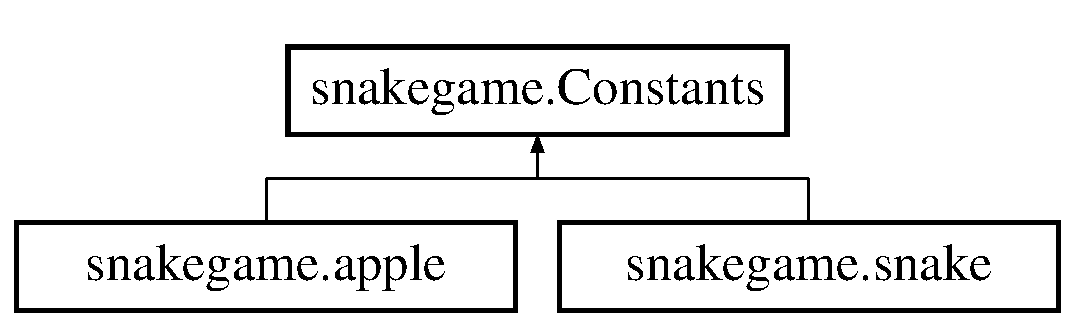
\includegraphics[height=2.000000cm]{classsnakegame_1_1_constants}
\end{center}
\end{figure}
\subsection*{Static Public Attributes}
\begin{DoxyCompactItemize}
\item 
static final int \mbox{\hyperlink{classsnakegame_1_1_constants_a253f00351ba8bbc4a7e7adf94ddd4a29}{B\+O\+R\+D\+E\+R\+\_\+\+W\+I\+D\+TH}} = 900
\item 
static final int \mbox{\hyperlink{classsnakegame_1_1_constants_a84c010eb1c979612c5b3627964f33385}{B\+O\+R\+D\+E\+R\+\_\+\+L\+E\+N\+G\+HT}} = 900
\item 
static final int \mbox{\hyperlink{classsnakegame_1_1_constants_a47ff3bd3c0ecae5e9f2b878915a9dad2}{UP}} = 1
\item 
static final int \mbox{\hyperlink{classsnakegame_1_1_constants_affe932cca510cf5d5f619af355a9e5e2}{R\+I\+G\+HT}} = 2
\item 
static final int \mbox{\hyperlink{classsnakegame_1_1_constants_ac9166aad2f05da4e80661a252c82f9f6}{D\+O\+WN}} = 3
\item 
static final int \mbox{\hyperlink{classsnakegame_1_1_constants_af2ce3ce8082b3922ef73a7cd291095d7}{L\+E\+FT}} = 4
\item 
static final int \mbox{\hyperlink{classsnakegame_1_1_constants_a112d1c18a610f11804c7e27734db6a40}{shift}} = 0
\item 
static final int \mbox{\hyperlink{classsnakegame_1_1_constants_a3c24c7aa6b732df3fd18eaf1394f9255}{step\+\_\+size}} = 20
\end{DoxyCompactItemize}


\subsection{Detailed Description}


Definition at line 3 of file Constants.\+java.



\subsection{Member Data Documentation}
\mbox{\Hypertarget{classsnakegame_1_1_constants_a84c010eb1c979612c5b3627964f33385}\label{classsnakegame_1_1_constants_a84c010eb1c979612c5b3627964f33385}} 
\index{snakegame\+::\+Constants@{snakegame\+::\+Constants}!B\+O\+R\+D\+E\+R\+\_\+\+L\+E\+N\+G\+HT@{B\+O\+R\+D\+E\+R\+\_\+\+L\+E\+N\+G\+HT}}
\index{B\+O\+R\+D\+E\+R\+\_\+\+L\+E\+N\+G\+HT@{B\+O\+R\+D\+E\+R\+\_\+\+L\+E\+N\+G\+HT}!snakegame\+::\+Constants@{snakegame\+::\+Constants}}
\subsubsection{\texorpdfstring{B\+O\+R\+D\+E\+R\+\_\+\+L\+E\+N\+G\+HT}{BORDER\_LENGHT}}
{\footnotesize\ttfamily final int snakegame.\+Constants.\+B\+O\+R\+D\+E\+R\+\_\+\+L\+E\+N\+G\+HT = 900\hspace{0.3cm}{\ttfamily [static]}}



Definition at line 5 of file Constants.\+java.

\mbox{\Hypertarget{classsnakegame_1_1_constants_a253f00351ba8bbc4a7e7adf94ddd4a29}\label{classsnakegame_1_1_constants_a253f00351ba8bbc4a7e7adf94ddd4a29}} 
\index{snakegame\+::\+Constants@{snakegame\+::\+Constants}!B\+O\+R\+D\+E\+R\+\_\+\+W\+I\+D\+TH@{B\+O\+R\+D\+E\+R\+\_\+\+W\+I\+D\+TH}}
\index{B\+O\+R\+D\+E\+R\+\_\+\+W\+I\+D\+TH@{B\+O\+R\+D\+E\+R\+\_\+\+W\+I\+D\+TH}!snakegame\+::\+Constants@{snakegame\+::\+Constants}}
\subsubsection{\texorpdfstring{B\+O\+R\+D\+E\+R\+\_\+\+W\+I\+D\+TH}{BORDER\_WIDTH}}
{\footnotesize\ttfamily final int snakegame.\+Constants.\+B\+O\+R\+D\+E\+R\+\_\+\+W\+I\+D\+TH = 900\hspace{0.3cm}{\ttfamily [static]}}



Definition at line 4 of file Constants.\+java.

\mbox{\Hypertarget{classsnakegame_1_1_constants_ac9166aad2f05da4e80661a252c82f9f6}\label{classsnakegame_1_1_constants_ac9166aad2f05da4e80661a252c82f9f6}} 
\index{snakegame\+::\+Constants@{snakegame\+::\+Constants}!D\+O\+WN@{D\+O\+WN}}
\index{D\+O\+WN@{D\+O\+WN}!snakegame\+::\+Constants@{snakegame\+::\+Constants}}
\subsubsection{\texorpdfstring{D\+O\+WN}{DOWN}}
{\footnotesize\ttfamily final int snakegame.\+Constants.\+D\+O\+WN = 3\hspace{0.3cm}{\ttfamily [static]}}



Definition at line 8 of file Constants.\+java.

\mbox{\Hypertarget{classsnakegame_1_1_constants_af2ce3ce8082b3922ef73a7cd291095d7}\label{classsnakegame_1_1_constants_af2ce3ce8082b3922ef73a7cd291095d7}} 
\index{snakegame\+::\+Constants@{snakegame\+::\+Constants}!L\+E\+FT@{L\+E\+FT}}
\index{L\+E\+FT@{L\+E\+FT}!snakegame\+::\+Constants@{snakegame\+::\+Constants}}
\subsubsection{\texorpdfstring{L\+E\+FT}{LEFT}}
{\footnotesize\ttfamily final int snakegame.\+Constants.\+L\+E\+FT = 4\hspace{0.3cm}{\ttfamily [static]}}



Definition at line 9 of file Constants.\+java.

\mbox{\Hypertarget{classsnakegame_1_1_constants_affe932cca510cf5d5f619af355a9e5e2}\label{classsnakegame_1_1_constants_affe932cca510cf5d5f619af355a9e5e2}} 
\index{snakegame\+::\+Constants@{snakegame\+::\+Constants}!R\+I\+G\+HT@{R\+I\+G\+HT}}
\index{R\+I\+G\+HT@{R\+I\+G\+HT}!snakegame\+::\+Constants@{snakegame\+::\+Constants}}
\subsubsection{\texorpdfstring{R\+I\+G\+HT}{RIGHT}}
{\footnotesize\ttfamily final int snakegame.\+Constants.\+R\+I\+G\+HT = 2\hspace{0.3cm}{\ttfamily [static]}}



Definition at line 7 of file Constants.\+java.

\mbox{\Hypertarget{classsnakegame_1_1_constants_a112d1c18a610f11804c7e27734db6a40}\label{classsnakegame_1_1_constants_a112d1c18a610f11804c7e27734db6a40}} 
\index{snakegame\+::\+Constants@{snakegame\+::\+Constants}!shift@{shift}}
\index{shift@{shift}!snakegame\+::\+Constants@{snakegame\+::\+Constants}}
\subsubsection{\texorpdfstring{shift}{shift}}
{\footnotesize\ttfamily final int snakegame.\+Constants.\+shift = 0\hspace{0.3cm}{\ttfamily [static]}}



Definition at line 10 of file Constants.\+java.

\mbox{\Hypertarget{classsnakegame_1_1_constants_a3c24c7aa6b732df3fd18eaf1394f9255}\label{classsnakegame_1_1_constants_a3c24c7aa6b732df3fd18eaf1394f9255}} 
\index{snakegame\+::\+Constants@{snakegame\+::\+Constants}!step\+\_\+size@{step\+\_\+size}}
\index{step\+\_\+size@{step\+\_\+size}!snakegame\+::\+Constants@{snakegame\+::\+Constants}}
\subsubsection{\texorpdfstring{step\+\_\+size}{step\_size}}
{\footnotesize\ttfamily final int snakegame.\+Constants.\+step\+\_\+size = 20\hspace{0.3cm}{\ttfamily [static]}}



Definition at line 11 of file Constants.\+java.

\mbox{\Hypertarget{classsnakegame_1_1_constants_a47ff3bd3c0ecae5e9f2b878915a9dad2}\label{classsnakegame_1_1_constants_a47ff3bd3c0ecae5e9f2b878915a9dad2}} 
\index{snakegame\+::\+Constants@{snakegame\+::\+Constants}!UP@{UP}}
\index{UP@{UP}!snakegame\+::\+Constants@{snakegame\+::\+Constants}}
\subsubsection{\texorpdfstring{UP}{UP}}
{\footnotesize\ttfamily final int snakegame.\+Constants.\+UP = 1\hspace{0.3cm}{\ttfamily [static]}}



Definition at line 6 of file Constants.\+java.



The documentation for this class was generated from the following file\+:\begin{DoxyCompactItemize}
\item 
src/snakegame/\mbox{\hyperlink{_constants_8java}{Constants.\+java}}\end{DoxyCompactItemize}

\hypertarget{classsnakegame_1_1server_1_1_contriols_queue}{}\section{snakegame.\+server.\+Contriols\+Queue Class Reference}
\label{classsnakegame_1_1server_1_1_contriols_queue}\index{snakegame.\+server.\+Contriols\+Queue@{snakegame.\+server.\+Contriols\+Queue}}


\subsection{Detailed Description}


Definition at line 6 of file Contriols\+Queue.\+java.



The documentation for this class was generated from the following file\+:\begin{DoxyCompactItemize}
\item 
src/snakegame/server/\mbox{\hyperlink{_contriols_queue_8java}{Contriols\+Queue.\+java}}\end{DoxyCompactItemize}

\hypertarget{enumsnakegame_1_1structs_1_1_direction}{}\section{snakegame.\+structs.\+Direction Enum Reference}
\label{enumsnakegame_1_1structs_1_1_direction}\index{snakegame.\+structs.\+Direction@{snakegame.\+structs.\+Direction}}
\subsection*{Public Member Functions}
\begin{DoxyCompactItemize}
\item 
\mbox{\hyperlink{enumsnakegame_1_1structs_1_1_direction}{Direction}} \mbox{\hyperlink{enumsnakegame_1_1structs_1_1_direction_a3f48c431df64ddc8d497746a14293fd7}{new\+Direction}} (Key\+Event event)
\item 
\mbox{\hyperlink{enumsnakegame_1_1structs_1_1_direction}{Direction}} \mbox{\hyperlink{enumsnakegame_1_1structs_1_1_direction_acca4af48b36042d85f1a9eab2becbf2a}{new\+Direction}} (int key\+Code)
\end{DoxyCompactItemize}
\subsection*{Public Attributes}
\begin{DoxyCompactItemize}
\item 
\mbox{\hyperlink{enumsnakegame_1_1structs_1_1_direction_a6eac992f122ba5b02aad12a7cfcf65ce}{up}}
\item 
\mbox{\hyperlink{enumsnakegame_1_1structs_1_1_direction_af5f078cc54af6fabd9325c39328c6d9c}{right}}
\item 
\mbox{\hyperlink{enumsnakegame_1_1structs_1_1_direction_ac1c479971b6ea1b25efe9d3eb82d1e46}{down}}
\end{DoxyCompactItemize}


\subsection{Detailed Description}


Definition at line 7 of file Direction.\+java.



\subsection{Member Function Documentation}
\mbox{\Hypertarget{enumsnakegame_1_1structs_1_1_direction_a3f48c431df64ddc8d497746a14293fd7}\label{enumsnakegame_1_1structs_1_1_direction_a3f48c431df64ddc8d497746a14293fd7}} 
\index{snakegame\+::structs\+::\+Direction@{snakegame\+::structs\+::\+Direction}!new\+Direction@{new\+Direction}}
\index{new\+Direction@{new\+Direction}!snakegame\+::structs\+::\+Direction@{snakegame\+::structs\+::\+Direction}}
\subsubsection{\texorpdfstring{new\+Direction()}{newDirection()}\hspace{0.1cm}{\footnotesize\ttfamily [1/2]}}
{\footnotesize\ttfamily \mbox{\hyperlink{enumsnakegame_1_1structs_1_1_direction}{Direction}} snakegame.\+structs.\+Direction.\+new\+Direction (\begin{DoxyParamCaption}\item[{Key\+Event}]{event }\end{DoxyParamCaption})}



Definition at line 14 of file Direction.\+java.

\mbox{\Hypertarget{enumsnakegame_1_1structs_1_1_direction_acca4af48b36042d85f1a9eab2becbf2a}\label{enumsnakegame_1_1structs_1_1_direction_acca4af48b36042d85f1a9eab2becbf2a}} 
\index{snakegame\+::structs\+::\+Direction@{snakegame\+::structs\+::\+Direction}!new\+Direction@{new\+Direction}}
\index{new\+Direction@{new\+Direction}!snakegame\+::structs\+::\+Direction@{snakegame\+::structs\+::\+Direction}}
\subsubsection{\texorpdfstring{new\+Direction()}{newDirection()}\hspace{0.1cm}{\footnotesize\ttfamily [2/2]}}
{\footnotesize\ttfamily \mbox{\hyperlink{enumsnakegame_1_1structs_1_1_direction}{Direction}} snakegame.\+structs.\+Direction.\+new\+Direction (\begin{DoxyParamCaption}\item[{int}]{key\+Code }\end{DoxyParamCaption})}



Definition at line 19 of file Direction.\+java.



\subsection{Member Data Documentation}
\mbox{\Hypertarget{enumsnakegame_1_1structs_1_1_direction_ac1c479971b6ea1b25efe9d3eb82d1e46}\label{enumsnakegame_1_1structs_1_1_direction_ac1c479971b6ea1b25efe9d3eb82d1e46}} 
\index{snakegame\+::structs\+::\+Direction@{snakegame\+::structs\+::\+Direction}!down@{down}}
\index{down@{down}!snakegame\+::structs\+::\+Direction@{snakegame\+::structs\+::\+Direction}}
\subsubsection{\texorpdfstring{down}{down}}
{\footnotesize\ttfamily snakegame.\+structs.\+Direction.\+down}



Definition at line 10 of file Direction.\+java.

\mbox{\Hypertarget{enumsnakegame_1_1structs_1_1_direction_af5f078cc54af6fabd9325c39328c6d9c}\label{enumsnakegame_1_1structs_1_1_direction_af5f078cc54af6fabd9325c39328c6d9c}} 
\index{snakegame\+::structs\+::\+Direction@{snakegame\+::structs\+::\+Direction}!right@{right}}
\index{right@{right}!snakegame\+::structs\+::\+Direction@{snakegame\+::structs\+::\+Direction}}
\subsubsection{\texorpdfstring{right}{right}}
{\footnotesize\ttfamily snakegame.\+structs.\+Direction.\+right}



Definition at line 9 of file Direction.\+java.

\mbox{\Hypertarget{enumsnakegame_1_1structs_1_1_direction_a6eac992f122ba5b02aad12a7cfcf65ce}\label{enumsnakegame_1_1structs_1_1_direction_a6eac992f122ba5b02aad12a7cfcf65ce}} 
\index{snakegame\+::structs\+::\+Direction@{snakegame\+::structs\+::\+Direction}!up@{up}}
\index{up@{up}!snakegame\+::structs\+::\+Direction@{snakegame\+::structs\+::\+Direction}}
\subsubsection{\texorpdfstring{up}{up}}
{\footnotesize\ttfamily snakegame.\+structs.\+Direction.\+up}



Definition at line 8 of file Direction.\+java.



The documentation for this enum was generated from the following file\+:\begin{DoxyCompactItemize}
\item 
src/snakegame/structs/\mbox{\hyperlink{_direction_8java}{Direction.\+java}}\end{DoxyCompactItemize}

\hypertarget{classsnakegame_1_1_game}{}\section{snakegame.\+Game Class Reference}
\label{classsnakegame_1_1_game}\index{snakegame.\+Game@{snakegame.\+Game}}
\subsection*{Static Public Member Functions}
\begin{DoxyCompactItemize}
\item 
static void \mbox{\hyperlink{classsnakegame_1_1_game_a5da8884fe16160449cf02f7c594b2f79}{main}} (String \mbox{[}$\,$\mbox{]} args)
\end{DoxyCompactItemize}


\subsection{Detailed Description}


Definition at line 8 of file Game.\+java.



\subsection{Member Function Documentation}
\mbox{\Hypertarget{classsnakegame_1_1_game_a5da8884fe16160449cf02f7c594b2f79}\label{classsnakegame_1_1_game_a5da8884fe16160449cf02f7c594b2f79}} 
\index{snakegame\+::\+Game@{snakegame\+::\+Game}!main@{main}}
\index{main@{main}!snakegame\+::\+Game@{snakegame\+::\+Game}}
\subsubsection{\texorpdfstring{main()}{main()}}
{\footnotesize\ttfamily static void snakegame.\+Game.\+main (\begin{DoxyParamCaption}\item[{String \mbox{[}$\,$\mbox{]}}]{args }\end{DoxyParamCaption})\hspace{0.3cm}{\ttfamily [static]}}



Definition at line 9 of file Game.\+java.



The documentation for this class was generated from the following file\+:\begin{DoxyCompactItemize}
\item 
src/snakegame/\mbox{\hyperlink{_game_8java}{Game.\+java}}\end{DoxyCompactItemize}

\hypertarget{classsnakegame_1_1_main_window}{}\section{snakegame.\+Main\+Window Class Reference}
\label{classsnakegame_1_1_main_window}\index{snakegame.\+Main\+Window@{snakegame.\+Main\+Window}}
Inheritance diagram for snakegame.\+Main\+Window\+:\begin{figure}[H]
\begin{center}
\leavevmode
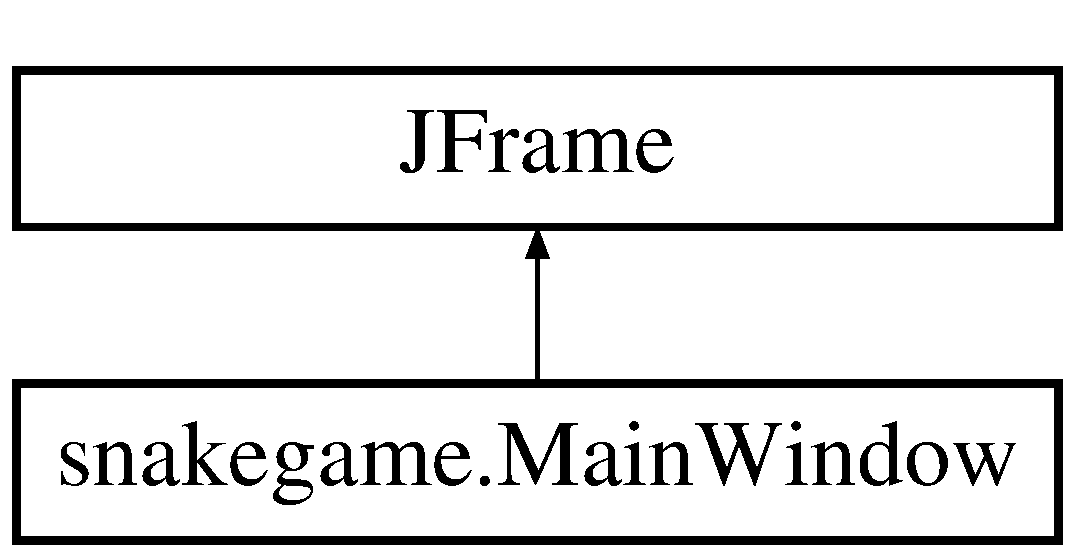
\includegraphics[height=2.000000cm]{classsnakegame_1_1_main_window}
\end{center}
\end{figure}
\subsection*{Public Member Functions}
\begin{DoxyCompactItemize}
\item 
void \mbox{\hyperlink{classsnakegame_1_1_main_window_ae412ac0550a3d9a165dc7ce7e5481ba3}{Input}} (Key\+Event event)
\item 
void \mbox{\hyperlink{classsnakegame_1_1_main_window_afe9dbd469853597ae9a61c56b85d2762}{paint}} (Graphics g)
\end{DoxyCompactItemize}


\subsection{Detailed Description}


Definition at line 11 of file Main\+Window.\+java.



\subsection{Member Function Documentation}
\mbox{\Hypertarget{classsnakegame_1_1_main_window_ae412ac0550a3d9a165dc7ce7e5481ba3}\label{classsnakegame_1_1_main_window_ae412ac0550a3d9a165dc7ce7e5481ba3}} 
\index{snakegame\+::\+Main\+Window@{snakegame\+::\+Main\+Window}!Input@{Input}}
\index{Input@{Input}!snakegame\+::\+Main\+Window@{snakegame\+::\+Main\+Window}}
\subsubsection{\texorpdfstring{Input()}{Input()}}
{\footnotesize\ttfamily void snakegame.\+Main\+Window.\+Input (\begin{DoxyParamCaption}\item[{Key\+Event}]{event }\end{DoxyParamCaption})}



Definition at line 61 of file Main\+Window.\+java.

\mbox{\Hypertarget{classsnakegame_1_1_main_window_afe9dbd469853597ae9a61c56b85d2762}\label{classsnakegame_1_1_main_window_afe9dbd469853597ae9a61c56b85d2762}} 
\index{snakegame\+::\+Main\+Window@{snakegame\+::\+Main\+Window}!paint@{paint}}
\index{paint@{paint}!snakegame\+::\+Main\+Window@{snakegame\+::\+Main\+Window}}
\subsubsection{\texorpdfstring{paint()}{paint()}}
{\footnotesize\ttfamily void snakegame.\+Main\+Window.\+paint (\begin{DoxyParamCaption}\item[{Graphics}]{g }\end{DoxyParamCaption})}



Definition at line 96 of file Main\+Window.\+java.



The documentation for this class was generated from the following file\+:\begin{DoxyCompactItemize}
\item 
src/snakegame/\mbox{\hyperlink{_main_window_8java}{Main\+Window.\+java}}\end{DoxyCompactItemize}

\hypertarget{classsnakegame_1_1server_1_1_message}{}\section{snakegame.\+server.\+Message Class Reference}
\label{classsnakegame_1_1server_1_1_message}\index{snakegame.\+server.\+Message@{snakegame.\+server.\+Message}}
\subsection*{Public Member Functions}
\begin{DoxyCompactItemize}
\item 
int \mbox{\hyperlink{classsnakegame_1_1server_1_1_message_ab530cae742ab3546af0531af6decfb4d}{get\+Key\+Code}} ()
\item 
U\+U\+ID \mbox{\hyperlink{classsnakegame_1_1server_1_1_message_a1813db6854615d0d545e7e7a24f73fe4}{get\+Uuid}} ()
\item 
\mbox{\hyperlink{classsnakegame_1_1server_1_1_message_a785c5537fe6e83fbc944dc86cc130db4}{Message}} (int key\+Code, U\+U\+ID uuid)
\item 
String \mbox{\hyperlink{classsnakegame_1_1server_1_1_message_a9e38b76d6815d73d7c14a28e8640b1c3}{to\+String}} ()
\end{DoxyCompactItemize}
\subsection*{Static Public Member Functions}
\begin{DoxyCompactItemize}
\item 
static \mbox{\hyperlink{classsnakegame_1_1server_1_1_message}{Message}} \mbox{\hyperlink{classsnakegame_1_1server_1_1_message_a18e375c0d7b140c6b4d141b870542a4a}{parse}} (String string)  throws Illegal\+Argument\+Exception 
\end{DoxyCompactItemize}


\subsection{Detailed Description}


Definition at line 7 of file Message.\+java.



\subsection{Constructor \& Destructor Documentation}
\mbox{\Hypertarget{classsnakegame_1_1server_1_1_message_a785c5537fe6e83fbc944dc86cc130db4}\label{classsnakegame_1_1server_1_1_message_a785c5537fe6e83fbc944dc86cc130db4}} 
\index{snakegame\+::server\+::\+Message@{snakegame\+::server\+::\+Message}!Message@{Message}}
\index{Message@{Message}!snakegame\+::server\+::\+Message@{snakegame\+::server\+::\+Message}}
\subsubsection{\texorpdfstring{Message()}{Message()}}
{\footnotesize\ttfamily snakegame.\+server.\+Message.\+Message (\begin{DoxyParamCaption}\item[{int}]{key\+Code,  }\item[{U\+U\+ID}]{uuid }\end{DoxyParamCaption})}



Definition at line 20 of file Message.\+java.



\subsection{Member Function Documentation}
\mbox{\Hypertarget{classsnakegame_1_1server_1_1_message_ab530cae742ab3546af0531af6decfb4d}\label{classsnakegame_1_1server_1_1_message_ab530cae742ab3546af0531af6decfb4d}} 
\index{snakegame\+::server\+::\+Message@{snakegame\+::server\+::\+Message}!get\+Key\+Code@{get\+Key\+Code}}
\index{get\+Key\+Code@{get\+Key\+Code}!snakegame\+::server\+::\+Message@{snakegame\+::server\+::\+Message}}
\subsubsection{\texorpdfstring{get\+Key\+Code()}{getKeyCode()}}
{\footnotesize\ttfamily int snakegame.\+server.\+Message.\+get\+Key\+Code (\begin{DoxyParamCaption}{ }\end{DoxyParamCaption})}



Definition at line 8 of file Message.\+java.

\mbox{\Hypertarget{classsnakegame_1_1server_1_1_message_a1813db6854615d0d545e7e7a24f73fe4}\label{classsnakegame_1_1server_1_1_message_a1813db6854615d0d545e7e7a24f73fe4}} 
\index{snakegame\+::server\+::\+Message@{snakegame\+::server\+::\+Message}!get\+Uuid@{get\+Uuid}}
\index{get\+Uuid@{get\+Uuid}!snakegame\+::server\+::\+Message@{snakegame\+::server\+::\+Message}}
\subsubsection{\texorpdfstring{get\+Uuid()}{getUuid()}}
{\footnotesize\ttfamily U\+U\+ID snakegame.\+server.\+Message.\+get\+Uuid (\begin{DoxyParamCaption}{ }\end{DoxyParamCaption})}



Definition at line 12 of file Message.\+java.

\mbox{\Hypertarget{classsnakegame_1_1server_1_1_message_a18e375c0d7b140c6b4d141b870542a4a}\label{classsnakegame_1_1server_1_1_message_a18e375c0d7b140c6b4d141b870542a4a}} 
\index{snakegame\+::server\+::\+Message@{snakegame\+::server\+::\+Message}!parse@{parse}}
\index{parse@{parse}!snakegame\+::server\+::\+Message@{snakegame\+::server\+::\+Message}}
\subsubsection{\texorpdfstring{parse()}{parse()}}
{\footnotesize\ttfamily static \mbox{\hyperlink{classsnakegame_1_1server_1_1_message}{Message}} snakegame.\+server.\+Message.\+parse (\begin{DoxyParamCaption}\item[{String}]{string }\end{DoxyParamCaption}) throws Illegal\+Argument\+Exception\hspace{0.3cm}{\ttfamily [static]}}



Definition at line 26 of file Message.\+java.

\mbox{\Hypertarget{classsnakegame_1_1server_1_1_message_a9e38b76d6815d73d7c14a28e8640b1c3}\label{classsnakegame_1_1server_1_1_message_a9e38b76d6815d73d7c14a28e8640b1c3}} 
\index{snakegame\+::server\+::\+Message@{snakegame\+::server\+::\+Message}!to\+String@{to\+String}}
\index{to\+String@{to\+String}!snakegame\+::server\+::\+Message@{snakegame\+::server\+::\+Message}}
\subsubsection{\texorpdfstring{to\+String()}{toString()}}
{\footnotesize\ttfamily String snakegame.\+server.\+Message.\+to\+String (\begin{DoxyParamCaption}{ }\end{DoxyParamCaption})}



Definition at line 35 of file Message.\+java.



The documentation for this class was generated from the following file\+:\begin{DoxyCompactItemize}
\item 
src/snakegame/server/\mbox{\hyperlink{_message_8java}{Message.\+java}}\end{DoxyCompactItemize}

\hypertarget{classsnakegame_1_1structs_1_1_point}{}\section{snakegame.\+structs.\+Point Class Reference}
\label{classsnakegame_1_1structs_1_1_point}\index{snakegame.\+structs.\+Point@{snakegame.\+structs.\+Point}}
Inheritance diagram for snakegame.\+structs.\+Point\+:\begin{figure}[H]
\begin{center}
\leavevmode
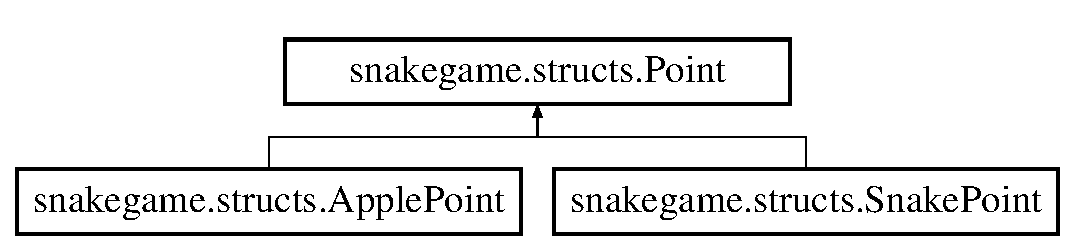
\includegraphics[height=2.000000cm]{classsnakegame_1_1structs_1_1_point}
\end{center}
\end{figure}
\subsection*{Public Member Functions}
\begin{DoxyCompactItemize}
\item 
\mbox{\hyperlink{classsnakegame_1_1structs_1_1_point_a79325ac308e18b3dd2721fcfa44752bd}{Point}} (\mbox{\hyperlink{classsnakegame_1_1structs_1_1_remainder}{Remainder}} \mbox{\hyperlink{classsnakegame_1_1structs_1_1_point_acf6c91ee7cda0e65a8054ff0dc07b79a}{x}}, \mbox{\hyperlink{classsnakegame_1_1structs_1_1_remainder}{Remainder}} \mbox{\hyperlink{classsnakegame_1_1structs_1_1_point_a2a9fe55d9cf57dbc120bbce39313d38d}{y}})
\item 
\mbox{\hyperlink{classsnakegame_1_1structs_1_1_remainder}{Remainder}} \mbox{\hyperlink{classsnakegame_1_1structs_1_1_point_a6dd8ef89102d12ec0cf5db0c03a568eb}{getX}} ()
\item 
void \mbox{\hyperlink{classsnakegame_1_1structs_1_1_point_a9efa9a335cccdbf667d1304c123e7ca9}{setX}} (\mbox{\hyperlink{classsnakegame_1_1structs_1_1_remainder}{Remainder}} \mbox{\hyperlink{classsnakegame_1_1structs_1_1_point_acf6c91ee7cda0e65a8054ff0dc07b79a}{x}})
\item 
\mbox{\hyperlink{classsnakegame_1_1structs_1_1_remainder}{Remainder}} \mbox{\hyperlink{classsnakegame_1_1structs_1_1_point_a920963cbc293b477335d7dc931ffb306}{getY}} ()
\item 
void \mbox{\hyperlink{classsnakegame_1_1structs_1_1_point_a9d42e4e18c765dcbfd14ef4baa102367}{setY}} (\mbox{\hyperlink{classsnakegame_1_1structs_1_1_remainder}{Remainder}} \mbox{\hyperlink{classsnakegame_1_1structs_1_1_point_a2a9fe55d9cf57dbc120bbce39313d38d}{y}})
\item 
abstract void \mbox{\hyperlink{classsnakegame_1_1structs_1_1_point_ab90de88df6692023c7e156d45f3e5417}{draw}} (Graphics2D g)
\item 
boolean \mbox{\hyperlink{classsnakegame_1_1structs_1_1_point_a46a08a1ffaa9cf65bab5527e620c0127}{equals}} (Object o)
\item 
int \mbox{\hyperlink{classsnakegame_1_1structs_1_1_point_a29332641bab79c8e403a6429d640e5f7}{hash\+Code}} ()
\item 
String \mbox{\hyperlink{classsnakegame_1_1structs_1_1_point_aec9ad3287697d952ab40687f5459241b}{to\+String}} ()
\end{DoxyCompactItemize}
\subsection*{Protected Attributes}
\begin{DoxyCompactItemize}
\item 
\mbox{\hyperlink{classsnakegame_1_1structs_1_1_remainder}{Remainder}} \mbox{\hyperlink{classsnakegame_1_1structs_1_1_point_acf6c91ee7cda0e65a8054ff0dc07b79a}{x}}
\item 
\mbox{\hyperlink{classsnakegame_1_1structs_1_1_remainder}{Remainder}} \mbox{\hyperlink{classsnakegame_1_1structs_1_1_point_a2a9fe55d9cf57dbc120bbce39313d38d}{y}}
\end{DoxyCompactItemize}


\subsection{Detailed Description}


Definition at line 5 of file Point.\+java.



\subsection{Constructor \& Destructor Documentation}
\mbox{\Hypertarget{classsnakegame_1_1structs_1_1_point_a79325ac308e18b3dd2721fcfa44752bd}\label{classsnakegame_1_1structs_1_1_point_a79325ac308e18b3dd2721fcfa44752bd}} 
\index{snakegame\+::structs\+::\+Point@{snakegame\+::structs\+::\+Point}!Point@{Point}}
\index{Point@{Point}!snakegame\+::structs\+::\+Point@{snakegame\+::structs\+::\+Point}}
\subsubsection{\texorpdfstring{Point()}{Point()}}
{\footnotesize\ttfamily snakegame.\+structs.\+Point.\+Point (\begin{DoxyParamCaption}\item[{\mbox{\hyperlink{classsnakegame_1_1structs_1_1_remainder}{Remainder}}}]{x,  }\item[{\mbox{\hyperlink{classsnakegame_1_1structs_1_1_remainder}{Remainder}}}]{y }\end{DoxyParamCaption})}



Definition at line 11 of file Point.\+java.



\subsection{Member Function Documentation}
\mbox{\Hypertarget{classsnakegame_1_1structs_1_1_point_ab90de88df6692023c7e156d45f3e5417}\label{classsnakegame_1_1structs_1_1_point_ab90de88df6692023c7e156d45f3e5417}} 
\index{snakegame\+::structs\+::\+Point@{snakegame\+::structs\+::\+Point}!draw@{draw}}
\index{draw@{draw}!snakegame\+::structs\+::\+Point@{snakegame\+::structs\+::\+Point}}
\subsubsection{\texorpdfstring{draw()}{draw()}}
{\footnotesize\ttfamily abstract void snakegame.\+structs.\+Point.\+draw (\begin{DoxyParamCaption}\item[{Graphics2D}]{g }\end{DoxyParamCaption})\hspace{0.3cm}{\ttfamily [abstract]}}

\mbox{\Hypertarget{classsnakegame_1_1structs_1_1_point_a46a08a1ffaa9cf65bab5527e620c0127}\label{classsnakegame_1_1structs_1_1_point_a46a08a1ffaa9cf65bab5527e620c0127}} 
\index{snakegame\+::structs\+::\+Point@{snakegame\+::structs\+::\+Point}!equals@{equals}}
\index{equals@{equals}!snakegame\+::structs\+::\+Point@{snakegame\+::structs\+::\+Point}}
\subsubsection{\texorpdfstring{equals()}{equals()}}
{\footnotesize\ttfamily boolean snakegame.\+structs.\+Point.\+equals (\begin{DoxyParamCaption}\item[{Object}]{o }\end{DoxyParamCaption})}



Definition at line 41 of file Point.\+java.

\mbox{\Hypertarget{classsnakegame_1_1structs_1_1_point_a6dd8ef89102d12ec0cf5db0c03a568eb}\label{classsnakegame_1_1structs_1_1_point_a6dd8ef89102d12ec0cf5db0c03a568eb}} 
\index{snakegame\+::structs\+::\+Point@{snakegame\+::structs\+::\+Point}!getX@{getX}}
\index{getX@{getX}!snakegame\+::structs\+::\+Point@{snakegame\+::structs\+::\+Point}}
\subsubsection{\texorpdfstring{get\+X()}{getX()}}
{\footnotesize\ttfamily \mbox{\hyperlink{classsnakegame_1_1structs_1_1_remainder}{Remainder}} snakegame.\+structs.\+Point.\+getX (\begin{DoxyParamCaption}{ }\end{DoxyParamCaption})}



Definition at line 17 of file Point.\+java.

\mbox{\Hypertarget{classsnakegame_1_1structs_1_1_point_a920963cbc293b477335d7dc931ffb306}\label{classsnakegame_1_1structs_1_1_point_a920963cbc293b477335d7dc931ffb306}} 
\index{snakegame\+::structs\+::\+Point@{snakegame\+::structs\+::\+Point}!getY@{getY}}
\index{getY@{getY}!snakegame\+::structs\+::\+Point@{snakegame\+::structs\+::\+Point}}
\subsubsection{\texorpdfstring{get\+Y()}{getY()}}
{\footnotesize\ttfamily \mbox{\hyperlink{classsnakegame_1_1structs_1_1_remainder}{Remainder}} snakegame.\+structs.\+Point.\+getY (\begin{DoxyParamCaption}{ }\end{DoxyParamCaption})}



Definition at line 27 of file Point.\+java.

\mbox{\Hypertarget{classsnakegame_1_1structs_1_1_point_a29332641bab79c8e403a6429d640e5f7}\label{classsnakegame_1_1structs_1_1_point_a29332641bab79c8e403a6429d640e5f7}} 
\index{snakegame\+::structs\+::\+Point@{snakegame\+::structs\+::\+Point}!hash\+Code@{hash\+Code}}
\index{hash\+Code@{hash\+Code}!snakegame\+::structs\+::\+Point@{snakegame\+::structs\+::\+Point}}
\subsubsection{\texorpdfstring{hash\+Code()}{hashCode()}}
{\footnotesize\ttfamily int snakegame.\+structs.\+Point.\+hash\+Code (\begin{DoxyParamCaption}{ }\end{DoxyParamCaption})}



Definition at line 53 of file Point.\+java.

\mbox{\Hypertarget{classsnakegame_1_1structs_1_1_point_a9efa9a335cccdbf667d1304c123e7ca9}\label{classsnakegame_1_1structs_1_1_point_a9efa9a335cccdbf667d1304c123e7ca9}} 
\index{snakegame\+::structs\+::\+Point@{snakegame\+::structs\+::\+Point}!setX@{setX}}
\index{setX@{setX}!snakegame\+::structs\+::\+Point@{snakegame\+::structs\+::\+Point}}
\subsubsection{\texorpdfstring{set\+X()}{setX()}}
{\footnotesize\ttfamily void snakegame.\+structs.\+Point.\+setX (\begin{DoxyParamCaption}\item[{\mbox{\hyperlink{classsnakegame_1_1structs_1_1_remainder}{Remainder}}}]{x }\end{DoxyParamCaption})}



Definition at line 22 of file Point.\+java.

\mbox{\Hypertarget{classsnakegame_1_1structs_1_1_point_a9d42e4e18c765dcbfd14ef4baa102367}\label{classsnakegame_1_1structs_1_1_point_a9d42e4e18c765dcbfd14ef4baa102367}} 
\index{snakegame\+::structs\+::\+Point@{snakegame\+::structs\+::\+Point}!setY@{setY}}
\index{setY@{setY}!snakegame\+::structs\+::\+Point@{snakegame\+::structs\+::\+Point}}
\subsubsection{\texorpdfstring{set\+Y()}{setY()}}
{\footnotesize\ttfamily void snakegame.\+structs.\+Point.\+setY (\begin{DoxyParamCaption}\item[{\mbox{\hyperlink{classsnakegame_1_1structs_1_1_remainder}{Remainder}}}]{y }\end{DoxyParamCaption})}



Definition at line 32 of file Point.\+java.

\mbox{\Hypertarget{classsnakegame_1_1structs_1_1_point_aec9ad3287697d952ab40687f5459241b}\label{classsnakegame_1_1structs_1_1_point_aec9ad3287697d952ab40687f5459241b}} 
\index{snakegame\+::structs\+::\+Point@{snakegame\+::structs\+::\+Point}!to\+String@{to\+String}}
\index{to\+String@{to\+String}!snakegame\+::structs\+::\+Point@{snakegame\+::structs\+::\+Point}}
\subsubsection{\texorpdfstring{to\+String()}{toString()}}
{\footnotesize\ttfamily String snakegame.\+structs.\+Point.\+to\+String (\begin{DoxyParamCaption}{ }\end{DoxyParamCaption})}



Definition at line 61 of file Point.\+java.



\subsection{Member Data Documentation}
\mbox{\Hypertarget{classsnakegame_1_1structs_1_1_point_acf6c91ee7cda0e65a8054ff0dc07b79a}\label{classsnakegame_1_1structs_1_1_point_acf6c91ee7cda0e65a8054ff0dc07b79a}} 
\index{snakegame\+::structs\+::\+Point@{snakegame\+::structs\+::\+Point}!x@{x}}
\index{x@{x}!snakegame\+::structs\+::\+Point@{snakegame\+::structs\+::\+Point}}
\subsubsection{\texorpdfstring{x}{x}}
{\footnotesize\ttfamily \mbox{\hyperlink{classsnakegame_1_1structs_1_1_remainder}{Remainder}} snakegame.\+structs.\+Point.\+x\hspace{0.3cm}{\ttfamily [protected]}}



Definition at line 6 of file Point.\+java.

\mbox{\Hypertarget{classsnakegame_1_1structs_1_1_point_a2a9fe55d9cf57dbc120bbce39313d38d}\label{classsnakegame_1_1structs_1_1_point_a2a9fe55d9cf57dbc120bbce39313d38d}} 
\index{snakegame\+::structs\+::\+Point@{snakegame\+::structs\+::\+Point}!y@{y}}
\index{y@{y}!snakegame\+::structs\+::\+Point@{snakegame\+::structs\+::\+Point}}
\subsubsection{\texorpdfstring{y}{y}}
{\footnotesize\ttfamily \mbox{\hyperlink{classsnakegame_1_1structs_1_1_remainder}{Remainder}} snakegame.\+structs.\+Point.\+y\hspace{0.3cm}{\ttfamily [protected]}}



Definition at line 7 of file Point.\+java.



The documentation for this class was generated from the following file\+:\begin{DoxyCompactItemize}
\item 
src/snakegame/structs/\mbox{\hyperlink{_point_8java}{Point.\+java}}\end{DoxyCompactItemize}

\hypertarget{classsnakegame_1_1structs_1_1_remainder}{}\section{snakegame.\+structs.\+Remainder Class Reference}
\label{classsnakegame_1_1structs_1_1_remainder}\index{snakegame.\+structs.\+Remainder@{snakegame.\+structs.\+Remainder}}
Inheritance diagram for snakegame.\+structs.\+Remainder\+:\begin{figure}[H]
\begin{center}
\leavevmode
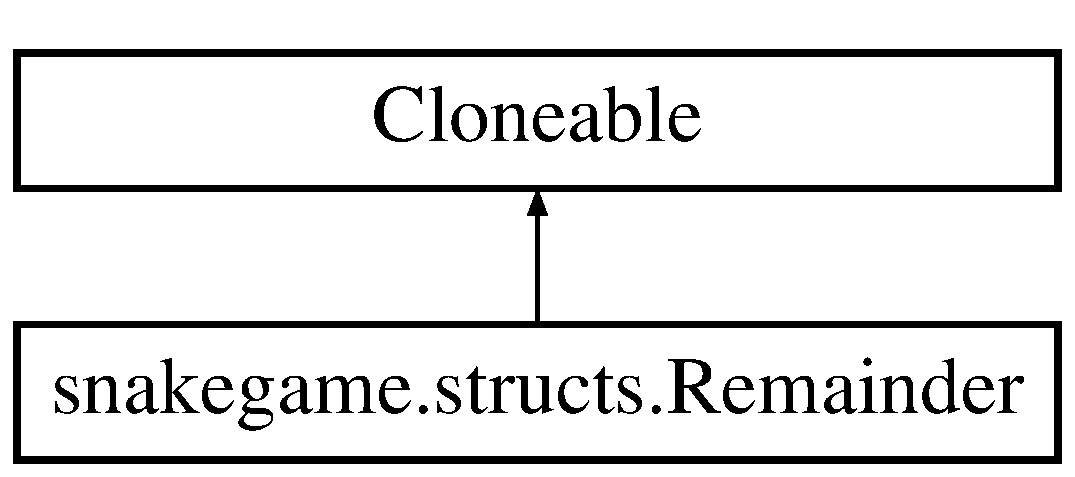
\includegraphics[height=2.000000cm]{classsnakegame_1_1structs_1_1_remainder}
\end{center}
\end{figure}
\subsection*{Public Member Functions}
\begin{DoxyCompactItemize}
\item 
\mbox{\hyperlink{classsnakegame_1_1structs_1_1_remainder_a5895859e2b9b2562a12a72495e316e9c}{Remainder}} (int limit, int value)
\item 
\mbox{\hyperlink{classsnakegame_1_1structs_1_1_remainder_ad01229fb264baa7f39848cb0c6db8afa}{Remainder}} (int value)
\item 
int \mbox{\hyperlink{classsnakegame_1_1structs_1_1_remainder_ad44771e1b21d1bd2ecb4b1f676395001}{get\+Value}} ()
\item 
void \mbox{\hyperlink{classsnakegame_1_1structs_1_1_remainder_ac280dde02bcc57ea35c8c7617cb57767}{set\+Value}} (int value)
\item 
\mbox{\hyperlink{classsnakegame_1_1structs_1_1_remainder}{Remainder}} \mbox{\hyperlink{classsnakegame_1_1structs_1_1_remainder_a3493d7ad668664ccd4089127794c4818}{copy}} ()
\item 
\mbox{\hyperlink{classsnakegame_1_1structs_1_1_remainder}{Remainder}} \mbox{\hyperlink{classsnakegame_1_1structs_1_1_remainder_a63bde400c1715836940db745a1e15f7f}{copy}} (int value)
\item 
\mbox{\hyperlink{classsnakegame_1_1structs_1_1_remainder}{Remainder}} \mbox{\hyperlink{classsnakegame_1_1structs_1_1_remainder_a0f899c321de31015e66951a3ea2cbcc3}{copy\+Add}} (int addition)
\item 
boolean \mbox{\hyperlink{classsnakegame_1_1structs_1_1_remainder_a5d11bc092dc689a2ddcff2947c27c679}{equals}} (Object o)
\item 
int \mbox{\hyperlink{classsnakegame_1_1structs_1_1_remainder_a65f6ae72c496323b19f05bbc93269127}{hash\+Code}} ()
\item 
String \mbox{\hyperlink{classsnakegame_1_1structs_1_1_remainder_a6d69e20d1a02d3feac7ce7873ed4d172}{to\+String}} ()
\end{DoxyCompactItemize}


\subsection{Detailed Description}


Definition at line 3 of file Remainder.\+java.



\subsection{Constructor \& Destructor Documentation}
\mbox{\Hypertarget{classsnakegame_1_1structs_1_1_remainder_a5895859e2b9b2562a12a72495e316e9c}\label{classsnakegame_1_1structs_1_1_remainder_a5895859e2b9b2562a12a72495e316e9c}} 
\index{snakegame\+::structs\+::\+Remainder@{snakegame\+::structs\+::\+Remainder}!Remainder@{Remainder}}
\index{Remainder@{Remainder}!snakegame\+::structs\+::\+Remainder@{snakegame\+::structs\+::\+Remainder}}
\subsubsection{\texorpdfstring{Remainder()}{Remainder()}\hspace{0.1cm}{\footnotesize\ttfamily [1/2]}}
{\footnotesize\ttfamily snakegame.\+structs.\+Remainder.\+Remainder (\begin{DoxyParamCaption}\item[{int}]{limit,  }\item[{int}]{value }\end{DoxyParamCaption})}



Definition at line 8 of file Remainder.\+java.

\mbox{\Hypertarget{classsnakegame_1_1structs_1_1_remainder_ad01229fb264baa7f39848cb0c6db8afa}\label{classsnakegame_1_1structs_1_1_remainder_ad01229fb264baa7f39848cb0c6db8afa}} 
\index{snakegame\+::structs\+::\+Remainder@{snakegame\+::structs\+::\+Remainder}!Remainder@{Remainder}}
\index{Remainder@{Remainder}!snakegame\+::structs\+::\+Remainder@{snakegame\+::structs\+::\+Remainder}}
\subsubsection{\texorpdfstring{Remainder()}{Remainder()}\hspace{0.1cm}{\footnotesize\ttfamily [2/2]}}
{\footnotesize\ttfamily snakegame.\+structs.\+Remainder.\+Remainder (\begin{DoxyParamCaption}\item[{int}]{value }\end{DoxyParamCaption})}



Definition at line 14 of file Remainder.\+java.



\subsection{Member Function Documentation}
\mbox{\Hypertarget{classsnakegame_1_1structs_1_1_remainder_a3493d7ad668664ccd4089127794c4818}\label{classsnakegame_1_1structs_1_1_remainder_a3493d7ad668664ccd4089127794c4818}} 
\index{snakegame\+::structs\+::\+Remainder@{snakegame\+::structs\+::\+Remainder}!copy@{copy}}
\index{copy@{copy}!snakegame\+::structs\+::\+Remainder@{snakegame\+::structs\+::\+Remainder}}
\subsubsection{\texorpdfstring{copy()}{copy()}\hspace{0.1cm}{\footnotesize\ttfamily [1/2]}}
{\footnotesize\ttfamily \mbox{\hyperlink{classsnakegame_1_1structs_1_1_remainder}{Remainder}} snakegame.\+structs.\+Remainder.\+copy (\begin{DoxyParamCaption}{ }\end{DoxyParamCaption})}



Definition at line 30 of file Remainder.\+java.

\mbox{\Hypertarget{classsnakegame_1_1structs_1_1_remainder_a63bde400c1715836940db745a1e15f7f}\label{classsnakegame_1_1structs_1_1_remainder_a63bde400c1715836940db745a1e15f7f}} 
\index{snakegame\+::structs\+::\+Remainder@{snakegame\+::structs\+::\+Remainder}!copy@{copy}}
\index{copy@{copy}!snakegame\+::structs\+::\+Remainder@{snakegame\+::structs\+::\+Remainder}}
\subsubsection{\texorpdfstring{copy()}{copy()}\hspace{0.1cm}{\footnotesize\ttfamily [2/2]}}
{\footnotesize\ttfamily \mbox{\hyperlink{classsnakegame_1_1structs_1_1_remainder}{Remainder}} snakegame.\+structs.\+Remainder.\+copy (\begin{DoxyParamCaption}\item[{int}]{value }\end{DoxyParamCaption})}



Definition at line 35 of file Remainder.\+java.

\mbox{\Hypertarget{classsnakegame_1_1structs_1_1_remainder_a0f899c321de31015e66951a3ea2cbcc3}\label{classsnakegame_1_1structs_1_1_remainder_a0f899c321de31015e66951a3ea2cbcc3}} 
\index{snakegame\+::structs\+::\+Remainder@{snakegame\+::structs\+::\+Remainder}!copy\+Add@{copy\+Add}}
\index{copy\+Add@{copy\+Add}!snakegame\+::structs\+::\+Remainder@{snakegame\+::structs\+::\+Remainder}}
\subsubsection{\texorpdfstring{copy\+Add()}{copyAdd()}}
{\footnotesize\ttfamily \mbox{\hyperlink{classsnakegame_1_1structs_1_1_remainder}{Remainder}} snakegame.\+structs.\+Remainder.\+copy\+Add (\begin{DoxyParamCaption}\item[{int}]{addition }\end{DoxyParamCaption})}



Definition at line 40 of file Remainder.\+java.

\mbox{\Hypertarget{classsnakegame_1_1structs_1_1_remainder_a5d11bc092dc689a2ddcff2947c27c679}\label{classsnakegame_1_1structs_1_1_remainder_a5d11bc092dc689a2ddcff2947c27c679}} 
\index{snakegame\+::structs\+::\+Remainder@{snakegame\+::structs\+::\+Remainder}!equals@{equals}}
\index{equals@{equals}!snakegame\+::structs\+::\+Remainder@{snakegame\+::structs\+::\+Remainder}}
\subsubsection{\texorpdfstring{equals()}{equals()}}
{\footnotesize\ttfamily boolean snakegame.\+structs.\+Remainder.\+equals (\begin{DoxyParamCaption}\item[{Object}]{o }\end{DoxyParamCaption})}



Definition at line 46 of file Remainder.\+java.

\mbox{\Hypertarget{classsnakegame_1_1structs_1_1_remainder_ad44771e1b21d1bd2ecb4b1f676395001}\label{classsnakegame_1_1structs_1_1_remainder_ad44771e1b21d1bd2ecb4b1f676395001}} 
\index{snakegame\+::structs\+::\+Remainder@{snakegame\+::structs\+::\+Remainder}!get\+Value@{get\+Value}}
\index{get\+Value@{get\+Value}!snakegame\+::structs\+::\+Remainder@{snakegame\+::structs\+::\+Remainder}}
\subsubsection{\texorpdfstring{get\+Value()}{getValue()}}
{\footnotesize\ttfamily int snakegame.\+structs.\+Remainder.\+get\+Value (\begin{DoxyParamCaption}{ }\end{DoxyParamCaption})}



Definition at line 20 of file Remainder.\+java.

\mbox{\Hypertarget{classsnakegame_1_1structs_1_1_remainder_a65f6ae72c496323b19f05bbc93269127}\label{classsnakegame_1_1structs_1_1_remainder_a65f6ae72c496323b19f05bbc93269127}} 
\index{snakegame\+::structs\+::\+Remainder@{snakegame\+::structs\+::\+Remainder}!hash\+Code@{hash\+Code}}
\index{hash\+Code@{hash\+Code}!snakegame\+::structs\+::\+Remainder@{snakegame\+::structs\+::\+Remainder}}
\subsubsection{\texorpdfstring{hash\+Code()}{hashCode()}}
{\footnotesize\ttfamily int snakegame.\+structs.\+Remainder.\+hash\+Code (\begin{DoxyParamCaption}{ }\end{DoxyParamCaption})}



Definition at line 58 of file Remainder.\+java.

\mbox{\Hypertarget{classsnakegame_1_1structs_1_1_remainder_ac280dde02bcc57ea35c8c7617cb57767}\label{classsnakegame_1_1structs_1_1_remainder_ac280dde02bcc57ea35c8c7617cb57767}} 
\index{snakegame\+::structs\+::\+Remainder@{snakegame\+::structs\+::\+Remainder}!set\+Value@{set\+Value}}
\index{set\+Value@{set\+Value}!snakegame\+::structs\+::\+Remainder@{snakegame\+::structs\+::\+Remainder}}
\subsubsection{\texorpdfstring{set\+Value()}{setValue()}}
{\footnotesize\ttfamily void snakegame.\+structs.\+Remainder.\+set\+Value (\begin{DoxyParamCaption}\item[{int}]{value }\end{DoxyParamCaption})}



Definition at line 25 of file Remainder.\+java.

\mbox{\Hypertarget{classsnakegame_1_1structs_1_1_remainder_a6d69e20d1a02d3feac7ce7873ed4d172}\label{classsnakegame_1_1structs_1_1_remainder_a6d69e20d1a02d3feac7ce7873ed4d172}} 
\index{snakegame\+::structs\+::\+Remainder@{snakegame\+::structs\+::\+Remainder}!to\+String@{to\+String}}
\index{to\+String@{to\+String}!snakegame\+::structs\+::\+Remainder@{snakegame\+::structs\+::\+Remainder}}
\subsubsection{\texorpdfstring{to\+String()}{toString()}}
{\footnotesize\ttfamily String snakegame.\+structs.\+Remainder.\+to\+String (\begin{DoxyParamCaption}{ }\end{DoxyParamCaption})}



Definition at line 65 of file Remainder.\+java.



The documentation for this class was generated from the following file\+:\begin{DoxyCompactItemize}
\item 
src/snakegame/structs/\mbox{\hyperlink{_remainder_8java}{Remainder.\+java}}\end{DoxyCompactItemize}

\hypertarget{classsnakegame_1_1server_1_1_server}{}\section{snakegame.\+server.\+Server Class Reference}
\label{classsnakegame_1_1server_1_1_server}\index{snakegame.\+server.\+Server@{snakegame.\+server.\+Server}}
\subsection*{Classes}
\begin{DoxyCompactItemize}
\item 
class \mbox{\hyperlink{classsnakegame_1_1server_1_1_server_1_1_client_handler}{Client\+Handler}}
\item 
class \mbox{\hyperlink{classsnakegame_1_1server_1_1_server_1_1_client_updater}{Client\+Updater}}
\item 
class \mbox{\hyperlink{classsnakegame_1_1server_1_1_server_1_1_world_updater}{World\+Updater}}
\end{DoxyCompactItemize}
\subsection*{Public Member Functions}
\begin{DoxyCompactItemize}
\item 
\mbox{\hyperlink{classsnakegame_1_1server_1_1_server_a483e80c850ea654902e0843f77eb783d}{Server}} (int port, String host)
\item 
\mbox{\hyperlink{classsnakegame_1_1server_1_1_server_a22825670547a8a66d0f0e8e48577101b}{Server}} ()
\item 
\mbox{\hyperlink{classsnakegame_1_1server_1_1_server_a2b8dd5769b5f1d9214a89856ff8923fd}{Server}} (int port)
\item 
\mbox{\hyperlink{classsnakegame_1_1server_1_1_server_af023d23576ddca43c378f1ce18273126}{Server}} (String host)
\item 
void \mbox{\hyperlink{classsnakegame_1_1server_1_1_server_af0101ad4e19f7ffc7ac541af737b5339}{run}} ()
\end{DoxyCompactItemize}
\subsection*{Static Public Member Functions}
\begin{DoxyCompactItemize}
\item 
static void \mbox{\hyperlink{classsnakegame_1_1server_1_1_server_ae7d47dbe33f4e0267a9a118c8541cd2d}{main}} (String\mbox{[}$\,$\mbox{]} args)
\end{DoxyCompactItemize}


\subsection{Detailed Description}


Definition at line 16 of file Server.\+java.



\subsection{Constructor \& Destructor Documentation}
\mbox{\Hypertarget{classsnakegame_1_1server_1_1_server_a483e80c850ea654902e0843f77eb783d}\label{classsnakegame_1_1server_1_1_server_a483e80c850ea654902e0843f77eb783d}} 
\index{snakegame\+::server\+::\+Server@{snakegame\+::server\+::\+Server}!Server@{Server}}
\index{Server@{Server}!snakegame\+::server\+::\+Server@{snakegame\+::server\+::\+Server}}
\subsubsection{\texorpdfstring{Server()}{Server()}\hspace{0.1cm}{\footnotesize\ttfamily [1/4]}}
{\footnotesize\ttfamily snakegame.\+server.\+Server.\+Server (\begin{DoxyParamCaption}\item[{int}]{port,  }\item[{String}]{host }\end{DoxyParamCaption})}



Definition at line 30 of file Server.\+java.

\mbox{\Hypertarget{classsnakegame_1_1server_1_1_server_a22825670547a8a66d0f0e8e48577101b}\label{classsnakegame_1_1server_1_1_server_a22825670547a8a66d0f0e8e48577101b}} 
\index{snakegame\+::server\+::\+Server@{snakegame\+::server\+::\+Server}!Server@{Server}}
\index{Server@{Server}!snakegame\+::server\+::\+Server@{snakegame\+::server\+::\+Server}}
\subsubsection{\texorpdfstring{Server()}{Server()}\hspace{0.1cm}{\footnotesize\ttfamily [2/4]}}
{\footnotesize\ttfamily snakegame.\+server.\+Server.\+Server (\begin{DoxyParamCaption}{ }\end{DoxyParamCaption})}



Definition at line 44 of file Server.\+java.

\mbox{\Hypertarget{classsnakegame_1_1server_1_1_server_a2b8dd5769b5f1d9214a89856ff8923fd}\label{classsnakegame_1_1server_1_1_server_a2b8dd5769b5f1d9214a89856ff8923fd}} 
\index{snakegame\+::server\+::\+Server@{snakegame\+::server\+::\+Server}!Server@{Server}}
\index{Server@{Server}!snakegame\+::server\+::\+Server@{snakegame\+::server\+::\+Server}}
\subsubsection{\texorpdfstring{Server()}{Server()}\hspace{0.1cm}{\footnotesize\ttfamily [3/4]}}
{\footnotesize\ttfamily snakegame.\+server.\+Server.\+Server (\begin{DoxyParamCaption}\item[{int}]{port }\end{DoxyParamCaption})}



Definition at line 49 of file Server.\+java.

\mbox{\Hypertarget{classsnakegame_1_1server_1_1_server_af023d23576ddca43c378f1ce18273126}\label{classsnakegame_1_1server_1_1_server_af023d23576ddca43c378f1ce18273126}} 
\index{snakegame\+::server\+::\+Server@{snakegame\+::server\+::\+Server}!Server@{Server}}
\index{Server@{Server}!snakegame\+::server\+::\+Server@{snakegame\+::server\+::\+Server}}
\subsubsection{\texorpdfstring{Server()}{Server()}\hspace{0.1cm}{\footnotesize\ttfamily [4/4]}}
{\footnotesize\ttfamily snakegame.\+server.\+Server.\+Server (\begin{DoxyParamCaption}\item[{String}]{host }\end{DoxyParamCaption})}



Definition at line 55 of file Server.\+java.



\subsection{Member Function Documentation}
\mbox{\Hypertarget{classsnakegame_1_1server_1_1_server_ae7d47dbe33f4e0267a9a118c8541cd2d}\label{classsnakegame_1_1server_1_1_server_ae7d47dbe33f4e0267a9a118c8541cd2d}} 
\index{snakegame\+::server\+::\+Server@{snakegame\+::server\+::\+Server}!main@{main}}
\index{main@{main}!snakegame\+::server\+::\+Server@{snakegame\+::server\+::\+Server}}
\subsubsection{\texorpdfstring{main()}{main()}}
{\footnotesize\ttfamily static void snakegame.\+server.\+Server.\+main (\begin{DoxyParamCaption}\item[{String \mbox{[}$\,$\mbox{]}}]{args }\end{DoxyParamCaption})\hspace{0.3cm}{\ttfamily [static]}}



Definition at line 77 of file Server.\+java.

\mbox{\Hypertarget{classsnakegame_1_1server_1_1_server_af0101ad4e19f7ffc7ac541af737b5339}\label{classsnakegame_1_1server_1_1_server_af0101ad4e19f7ffc7ac541af737b5339}} 
\index{snakegame\+::server\+::\+Server@{snakegame\+::server\+::\+Server}!run@{run}}
\index{run@{run}!snakegame\+::server\+::\+Server@{snakegame\+::server\+::\+Server}}
\subsubsection{\texorpdfstring{run()}{run()}}
{\footnotesize\ttfamily void snakegame.\+server.\+Server.\+run (\begin{DoxyParamCaption}{ }\end{DoxyParamCaption})}



Definition at line 60 of file Server.\+java.



The documentation for this class was generated from the following file\+:\begin{DoxyCompactItemize}
\item 
src/snakegame/server/\mbox{\hyperlink{_server_8java}{Server.\+java}}\end{DoxyCompactItemize}

\hypertarget{classsnakegame_1_1structs_1_1_snake}{}\section{snakegame.\+structs.\+Snake Class Reference}
\label{classsnakegame_1_1structs_1_1_snake}\index{snakegame.\+structs.\+Snake@{snakegame.\+structs.\+Snake}}
\subsection*{Public Member Functions}
\begin{DoxyCompactItemize}
\item 
U\+U\+ID \mbox{\hyperlink{classsnakegame_1_1structs_1_1_snake_ac17bff959740ffec977a37b6ed905a0c}{get\+Uuid}} ()
\item 
List$<$ \mbox{\hyperlink{classsnakegame_1_1structs_1_1_point}{Point}} $>$ \mbox{\hyperlink{classsnakegame_1_1structs_1_1_snake_a1201fceabdd51b2cbb3fdd69f151fec9}{get\+Points}} ()
\item 
\mbox{\hyperlink{classsnakegame_1_1structs_1_1_snake_ae76efb0ea42951d99b3f3e3134622120}{Snake}} (Linked\+List$<$ \mbox{\hyperlink{classsnakegame_1_1structs_1_1_point}{Point}} $>$ points, \mbox{\hyperlink{enumsnakegame_1_1structs_1_1_direction}{Direction}} direction)
\item 
\mbox{\hyperlink{classsnakegame_1_1structs_1_1_snake_afae60310456b2ff1474879d2c80d75b1}{Snake}} (U\+U\+ID uuid, Linked\+List$<$ \mbox{\hyperlink{classsnakegame_1_1structs_1_1_point}{Point}} $>$ points, \mbox{\hyperlink{enumsnakegame_1_1structs_1_1_direction}{Direction}} direction)
\item 
\mbox{\hyperlink{classsnakegame_1_1structs_1_1_snake_a4d2bf8212dfe91b17aed31f44203f37f}{Snake}} (\mbox{\hyperlink{classsnakegame_1_1structs_1_1_snake}{Snake}} \mbox{\hyperlink{classsnakegame_1_1snake}{snake}})
\item 
\mbox{\hyperlink{classsnakegame_1_1structs_1_1_snake}{Snake}} \mbox{\hyperlink{classsnakegame_1_1structs_1_1_snake_a0e8e4b28dd22705782f7a985e17b364d}{predict\+Move}} ()
\item 
\mbox{\hyperlink{enumsnakegame_1_1structs_1_1_direction}{Direction}} \mbox{\hyperlink{classsnakegame_1_1structs_1_1_snake_a596ece3775ed531cef2fc023f339052e}{get\+Direction}} ()
\item 
void \mbox{\hyperlink{classsnakegame_1_1structs_1_1_snake_abcd015387736c76d4c6770cb7d33f59c}{set\+Direction}} (\mbox{\hyperlink{enumsnakegame_1_1structs_1_1_direction}{Direction}} direction)
\item 
\mbox{\hyperlink{classsnakegame_1_1structs_1_1_point}{Point}} \mbox{\hyperlink{classsnakegame_1_1structs_1_1_snake_a75d7bc3f6202e0159e79b703fdd5232c}{get\+Head}} ()
\item 
boolean \mbox{\hyperlink{classsnakegame_1_1structs_1_1_snake_a3df7436c11ba7bda4154431739778b78}{contains}} (\mbox{\hyperlink{classsnakegame_1_1structs_1_1_point}{Point}} another\+Point)
\item 
boolean \mbox{\hyperlink{classsnakegame_1_1structs_1_1_snake_acefd74708c76a65a7e9f8e5182ae3af3}{ate\+Self}} ()
\item 
void \mbox{\hyperlink{classsnakegame_1_1structs_1_1_snake_a4e147dbd9e7442dce1b4f066946f8959}{move\+Head}} ()
\item 
void \mbox{\hyperlink{classsnakegame_1_1structs_1_1_snake_aefdd30421bce904e5585dbcbec258a98}{draw}} (Graphics2D g)
\item 
String \mbox{\hyperlink{classsnakegame_1_1structs_1_1_snake_a7ebadfc8fb3f4b24d0de3a6b3bde703e}{to\+String}} ()
\end{DoxyCompactItemize}
\subsection*{Static Public Member Functions}
\begin{DoxyCompactItemize}
\item 
static \mbox{\hyperlink{classsnakegame_1_1structs_1_1_snake}{Snake}} \mbox{\hyperlink{classsnakegame_1_1structs_1_1_snake_a5c7858e4b58db59e493b12c18462fb4b}{parse}} (String string)  throws Illegal\+Argument\+Exception 
\end{DoxyCompactItemize}


\subsection{Detailed Description}


Definition at line 7 of file Snake.\+java.



\subsection{Constructor \& Destructor Documentation}
\mbox{\Hypertarget{classsnakegame_1_1structs_1_1_snake_ae76efb0ea42951d99b3f3e3134622120}\label{classsnakegame_1_1structs_1_1_snake_ae76efb0ea42951d99b3f3e3134622120}} 
\index{snakegame\+::structs\+::\+Snake@{snakegame\+::structs\+::\+Snake}!Snake@{Snake}}
\index{Snake@{Snake}!snakegame\+::structs\+::\+Snake@{snakegame\+::structs\+::\+Snake}}
\subsubsection{\texorpdfstring{Snake()}{Snake()}\hspace{0.1cm}{\footnotesize\ttfamily [1/3]}}
{\footnotesize\ttfamily snakegame.\+structs.\+Snake.\+Snake (\begin{DoxyParamCaption}\item[{Linked\+List$<$ \mbox{\hyperlink{classsnakegame_1_1structs_1_1_point}{Point}} $>$}]{points,  }\item[{\mbox{\hyperlink{enumsnakegame_1_1structs_1_1_direction}{Direction}}}]{direction }\end{DoxyParamCaption})}



Definition at line 23 of file Snake.\+java.

\mbox{\Hypertarget{classsnakegame_1_1structs_1_1_snake_afae60310456b2ff1474879d2c80d75b1}\label{classsnakegame_1_1structs_1_1_snake_afae60310456b2ff1474879d2c80d75b1}} 
\index{snakegame\+::structs\+::\+Snake@{snakegame\+::structs\+::\+Snake}!Snake@{Snake}}
\index{Snake@{Snake}!snakegame\+::structs\+::\+Snake@{snakegame\+::structs\+::\+Snake}}
\subsubsection{\texorpdfstring{Snake()}{Snake()}\hspace{0.1cm}{\footnotesize\ttfamily [2/3]}}
{\footnotesize\ttfamily snakegame.\+structs.\+Snake.\+Snake (\begin{DoxyParamCaption}\item[{U\+U\+ID}]{uuid,  }\item[{Linked\+List$<$ \mbox{\hyperlink{classsnakegame_1_1structs_1_1_point}{Point}} $>$}]{points,  }\item[{\mbox{\hyperlink{enumsnakegame_1_1structs_1_1_direction}{Direction}}}]{direction }\end{DoxyParamCaption})}



Definition at line 30 of file Snake.\+java.

\mbox{\Hypertarget{classsnakegame_1_1structs_1_1_snake_a4d2bf8212dfe91b17aed31f44203f37f}\label{classsnakegame_1_1structs_1_1_snake_a4d2bf8212dfe91b17aed31f44203f37f}} 
\index{snakegame\+::structs\+::\+Snake@{snakegame\+::structs\+::\+Snake}!Snake@{Snake}}
\index{Snake@{Snake}!snakegame\+::structs\+::\+Snake@{snakegame\+::structs\+::\+Snake}}
\subsubsection{\texorpdfstring{Snake()}{Snake()}\hspace{0.1cm}{\footnotesize\ttfamily [3/3]}}
{\footnotesize\ttfamily snakegame.\+structs.\+Snake.\+Snake (\begin{DoxyParamCaption}\item[{\mbox{\hyperlink{classsnakegame_1_1structs_1_1_snake}{Snake}}}]{snake }\end{DoxyParamCaption})}



Definition at line 37 of file Snake.\+java.



\subsection{Member Function Documentation}
\mbox{\Hypertarget{classsnakegame_1_1structs_1_1_snake_acefd74708c76a65a7e9f8e5182ae3af3}\label{classsnakegame_1_1structs_1_1_snake_acefd74708c76a65a7e9f8e5182ae3af3}} 
\index{snakegame\+::structs\+::\+Snake@{snakegame\+::structs\+::\+Snake}!ate\+Self@{ate\+Self}}
\index{ate\+Self@{ate\+Self}!snakegame\+::structs\+::\+Snake@{snakegame\+::structs\+::\+Snake}}
\subsubsection{\texorpdfstring{ate\+Self()}{ateSelf()}}
{\footnotesize\ttfamily boolean snakegame.\+structs.\+Snake.\+ate\+Self (\begin{DoxyParamCaption}{ }\end{DoxyParamCaption})}



Definition at line 76 of file Snake.\+java.

\mbox{\Hypertarget{classsnakegame_1_1structs_1_1_snake_a3df7436c11ba7bda4154431739778b78}\label{classsnakegame_1_1structs_1_1_snake_a3df7436c11ba7bda4154431739778b78}} 
\index{snakegame\+::structs\+::\+Snake@{snakegame\+::structs\+::\+Snake}!contains@{contains}}
\index{contains@{contains}!snakegame\+::structs\+::\+Snake@{snakegame\+::structs\+::\+Snake}}
\subsubsection{\texorpdfstring{contains()}{contains()}}
{\footnotesize\ttfamily boolean snakegame.\+structs.\+Snake.\+contains (\begin{DoxyParamCaption}\item[{\mbox{\hyperlink{classsnakegame_1_1structs_1_1_point}{Point}}}]{another\+Point }\end{DoxyParamCaption})}



Definition at line 66 of file Snake.\+java.

\mbox{\Hypertarget{classsnakegame_1_1structs_1_1_snake_aefdd30421bce904e5585dbcbec258a98}\label{classsnakegame_1_1structs_1_1_snake_aefdd30421bce904e5585dbcbec258a98}} 
\index{snakegame\+::structs\+::\+Snake@{snakegame\+::structs\+::\+Snake}!draw@{draw}}
\index{draw@{draw}!snakegame\+::structs\+::\+Snake@{snakegame\+::structs\+::\+Snake}}
\subsubsection{\texorpdfstring{draw()}{draw()}}
{\footnotesize\ttfamily void snakegame.\+structs.\+Snake.\+draw (\begin{DoxyParamCaption}\item[{Graphics2D}]{g }\end{DoxyParamCaption})}



Definition at line 142 of file Snake.\+java.

\mbox{\Hypertarget{classsnakegame_1_1structs_1_1_snake_a596ece3775ed531cef2fc023f339052e}\label{classsnakegame_1_1structs_1_1_snake_a596ece3775ed531cef2fc023f339052e}} 
\index{snakegame\+::structs\+::\+Snake@{snakegame\+::structs\+::\+Snake}!get\+Direction@{get\+Direction}}
\index{get\+Direction@{get\+Direction}!snakegame\+::structs\+::\+Snake@{snakegame\+::structs\+::\+Snake}}
\subsubsection{\texorpdfstring{get\+Direction()}{getDirection()}}
{\footnotesize\ttfamily \mbox{\hyperlink{enumsnakegame_1_1structs_1_1_direction}{Direction}} snakegame.\+structs.\+Snake.\+get\+Direction (\begin{DoxyParamCaption}{ }\end{DoxyParamCaption})}



Definition at line 51 of file Snake.\+java.

\mbox{\Hypertarget{classsnakegame_1_1structs_1_1_snake_a75d7bc3f6202e0159e79b703fdd5232c}\label{classsnakegame_1_1structs_1_1_snake_a75d7bc3f6202e0159e79b703fdd5232c}} 
\index{snakegame\+::structs\+::\+Snake@{snakegame\+::structs\+::\+Snake}!get\+Head@{get\+Head}}
\index{get\+Head@{get\+Head}!snakegame\+::structs\+::\+Snake@{snakegame\+::structs\+::\+Snake}}
\subsubsection{\texorpdfstring{get\+Head()}{getHead()}}
{\footnotesize\ttfamily \mbox{\hyperlink{classsnakegame_1_1structs_1_1_point}{Point}} snakegame.\+structs.\+Snake.\+get\+Head (\begin{DoxyParamCaption}{ }\end{DoxyParamCaption})}



Definition at line 61 of file Snake.\+java.

\mbox{\Hypertarget{classsnakegame_1_1structs_1_1_snake_a1201fceabdd51b2cbb3fdd69f151fec9}\label{classsnakegame_1_1structs_1_1_snake_a1201fceabdd51b2cbb3fdd69f151fec9}} 
\index{snakegame\+::structs\+::\+Snake@{snakegame\+::structs\+::\+Snake}!get\+Points@{get\+Points}}
\index{get\+Points@{get\+Points}!snakegame\+::structs\+::\+Snake@{snakegame\+::structs\+::\+Snake}}
\subsubsection{\texorpdfstring{get\+Points()}{getPoints()}}
{\footnotesize\ttfamily List$<$\mbox{\hyperlink{classsnakegame_1_1structs_1_1_point}{Point}}$>$ snakegame.\+structs.\+Snake.\+get\+Points (\begin{DoxyParamCaption}{ }\end{DoxyParamCaption})}



Definition at line 14 of file Snake.\+java.

\mbox{\Hypertarget{classsnakegame_1_1structs_1_1_snake_ac17bff959740ffec977a37b6ed905a0c}\label{classsnakegame_1_1structs_1_1_snake_ac17bff959740ffec977a37b6ed905a0c}} 
\index{snakegame\+::structs\+::\+Snake@{snakegame\+::structs\+::\+Snake}!get\+Uuid@{get\+Uuid}}
\index{get\+Uuid@{get\+Uuid}!snakegame\+::structs\+::\+Snake@{snakegame\+::structs\+::\+Snake}}
\subsubsection{\texorpdfstring{get\+Uuid()}{getUuid()}}
{\footnotesize\ttfamily U\+U\+ID snakegame.\+structs.\+Snake.\+get\+Uuid (\begin{DoxyParamCaption}{ }\end{DoxyParamCaption})}



Definition at line 8 of file Snake.\+java.

\mbox{\Hypertarget{classsnakegame_1_1structs_1_1_snake_a4e147dbd9e7442dce1b4f066946f8959}\label{classsnakegame_1_1structs_1_1_snake_a4e147dbd9e7442dce1b4f066946f8959}} 
\index{snakegame\+::structs\+::\+Snake@{snakegame\+::structs\+::\+Snake}!move\+Head@{move\+Head}}
\index{move\+Head@{move\+Head}!snakegame\+::structs\+::\+Snake@{snakegame\+::structs\+::\+Snake}}
\subsubsection{\texorpdfstring{move\+Head()}{moveHead()}}
{\footnotesize\ttfamily void snakegame.\+structs.\+Snake.\+move\+Head (\begin{DoxyParamCaption}{ }\end{DoxyParamCaption})}



Definition at line 95 of file Snake.\+java.

\mbox{\Hypertarget{classsnakegame_1_1structs_1_1_snake_a5c7858e4b58db59e493b12c18462fb4b}\label{classsnakegame_1_1structs_1_1_snake_a5c7858e4b58db59e493b12c18462fb4b}} 
\index{snakegame\+::structs\+::\+Snake@{snakegame\+::structs\+::\+Snake}!parse@{parse}}
\index{parse@{parse}!snakegame\+::structs\+::\+Snake@{snakegame\+::structs\+::\+Snake}}
\subsubsection{\texorpdfstring{parse()}{parse()}}
{\footnotesize\ttfamily static \mbox{\hyperlink{classsnakegame_1_1structs_1_1_snake}{Snake}} snakegame.\+structs.\+Snake.\+parse (\begin{DoxyParamCaption}\item[{String}]{string }\end{DoxyParamCaption}) throws Illegal\+Argument\+Exception\hspace{0.3cm}{\ttfamily [static]}}



Definition at line 118 of file Snake.\+java.

\mbox{\Hypertarget{classsnakegame_1_1structs_1_1_snake_a0e8e4b28dd22705782f7a985e17b364d}\label{classsnakegame_1_1structs_1_1_snake_a0e8e4b28dd22705782f7a985e17b364d}} 
\index{snakegame\+::structs\+::\+Snake@{snakegame\+::structs\+::\+Snake}!predict\+Move@{predict\+Move}}
\index{predict\+Move@{predict\+Move}!snakegame\+::structs\+::\+Snake@{snakegame\+::structs\+::\+Snake}}
\subsubsection{\texorpdfstring{predict\+Move()}{predictMove()}}
{\footnotesize\ttfamily \mbox{\hyperlink{classsnakegame_1_1structs_1_1_snake}{Snake}} snakegame.\+structs.\+Snake.\+predict\+Move (\begin{DoxyParamCaption}{ }\end{DoxyParamCaption})}



Definition at line 44 of file Snake.\+java.

\mbox{\Hypertarget{classsnakegame_1_1structs_1_1_snake_abcd015387736c76d4c6770cb7d33f59c}\label{classsnakegame_1_1structs_1_1_snake_abcd015387736c76d4c6770cb7d33f59c}} 
\index{snakegame\+::structs\+::\+Snake@{snakegame\+::structs\+::\+Snake}!set\+Direction@{set\+Direction}}
\index{set\+Direction@{set\+Direction}!snakegame\+::structs\+::\+Snake@{snakegame\+::structs\+::\+Snake}}
\subsubsection{\texorpdfstring{set\+Direction()}{setDirection()}}
{\footnotesize\ttfamily void snakegame.\+structs.\+Snake.\+set\+Direction (\begin{DoxyParamCaption}\item[{\mbox{\hyperlink{enumsnakegame_1_1structs_1_1_direction}{Direction}}}]{direction }\end{DoxyParamCaption})}



Definition at line 56 of file Snake.\+java.

\mbox{\Hypertarget{classsnakegame_1_1structs_1_1_snake_a7ebadfc8fb3f4b24d0de3a6b3bde703e}\label{classsnakegame_1_1structs_1_1_snake_a7ebadfc8fb3f4b24d0de3a6b3bde703e}} 
\index{snakegame\+::structs\+::\+Snake@{snakegame\+::structs\+::\+Snake}!to\+String@{to\+String}}
\index{to\+String@{to\+String}!snakegame\+::structs\+::\+Snake@{snakegame\+::structs\+::\+Snake}}
\subsubsection{\texorpdfstring{to\+String()}{toString()}}
{\footnotesize\ttfamily String snakegame.\+structs.\+Snake.\+to\+String (\begin{DoxyParamCaption}{ }\end{DoxyParamCaption})}



Definition at line 149 of file Snake.\+java.



The documentation for this class was generated from the following file\+:\begin{DoxyCompactItemize}
\item 
src/snakegame/structs/\mbox{\hyperlink{structs_2snake_8java}{Snake.\+java}}\end{DoxyCompactItemize}

\hypertarget{classsnakegame_1_1snake}{}\section{snakegame.\+snake Class Reference}
\label{classsnakegame_1_1snake}\index{snakegame.\+snake@{snakegame.\+snake}}
Inheritance diagram for snakegame.\+snake\+:\begin{figure}[H]
\begin{center}
\leavevmode
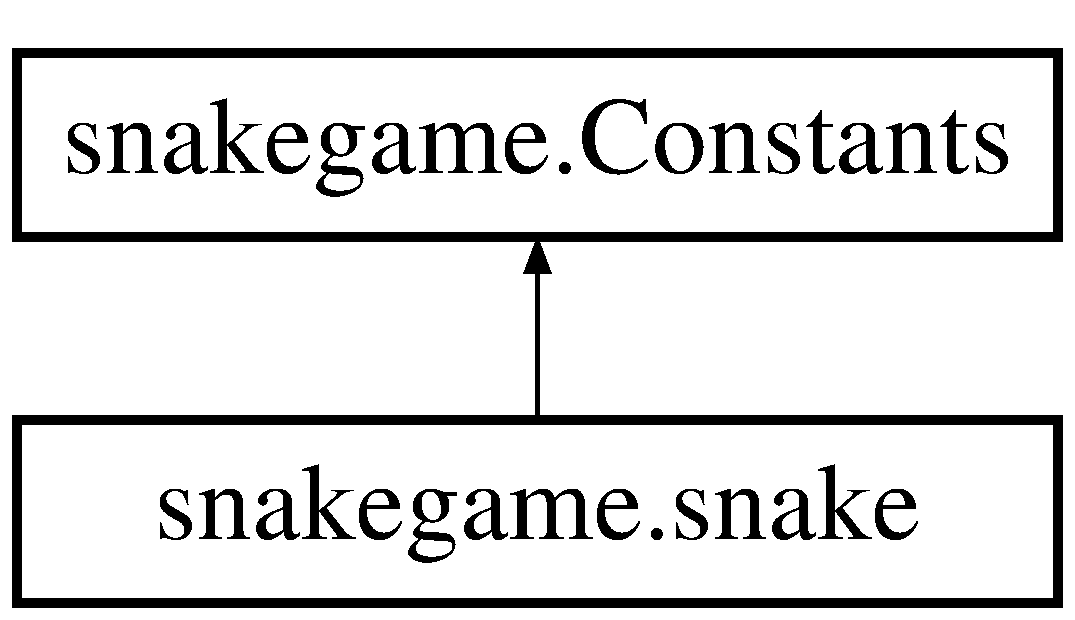
\includegraphics[height=2.000000cm]{classsnakegame_1_1snake}
\end{center}
\end{figure}
\subsection*{Public Member Functions}
\begin{DoxyCompactItemize}
\item 
int \mbox{\hyperlink{classsnakegame_1_1snake_a488d8293668de46cd8daf048d26a2b55}{get\+Direction}} ()
\item 
void \mbox{\hyperlink{classsnakegame_1_1snake_ad2d7f86bae0fc94adde6c4417b4e1b8a}{set\+Direction}} (int direction)
\item 
Point \mbox{\hyperlink{classsnakegame_1_1snake_a1f9f29ffc498ba715fbb5419f35bc7fa}{head}} ()
\item 
Array\+List$<$ Point $>$ \mbox{\hyperlink{classsnakegame_1_1snake_a63cca0235c21cd483d69bb52e17d48cf}{body}} ()
\item 
void \mbox{\hyperlink{classsnakegame_1_1snake_a9372b56db6a2e802f5bb7e7fc1b244d5}{logic}} ()
\item 
void \mbox{\hyperlink{classsnakegame_1_1snake_a0997b6e2c2b622c3f4b013868c0165b1}{paint}} (Graphics2D g2)
\end{DoxyCompactItemize}
\subsection*{Additional Inherited Members}


\subsection{Detailed Description}


Definition at line 9 of file snake.\+java.



\subsection{Member Function Documentation}
\mbox{\Hypertarget{classsnakegame_1_1snake_a63cca0235c21cd483d69bb52e17d48cf}\label{classsnakegame_1_1snake_a63cca0235c21cd483d69bb52e17d48cf}} 
\index{snakegame\+::snake@{snakegame\+::snake}!body@{body}}
\index{body@{body}!snakegame\+::snake@{snakegame\+::snake}}
\subsubsection{\texorpdfstring{body()}{body()}}
{\footnotesize\ttfamily Array\+List$<$Point$>$ snakegame.\+snake.\+body (\begin{DoxyParamCaption}{ }\end{DoxyParamCaption})}



Definition at line 44 of file snake.\+java.

\mbox{\Hypertarget{classsnakegame_1_1snake_a488d8293668de46cd8daf048d26a2b55}\label{classsnakegame_1_1snake_a488d8293668de46cd8daf048d26a2b55}} 
\index{snakegame\+::snake@{snakegame\+::snake}!get\+Direction@{get\+Direction}}
\index{get\+Direction@{get\+Direction}!snakegame\+::snake@{snakegame\+::snake}}
\subsubsection{\texorpdfstring{get\+Direction()}{getDirection()}}
{\footnotesize\ttfamily int snakegame.\+snake.\+get\+Direction (\begin{DoxyParamCaption}{ }\end{DoxyParamCaption})}



Definition at line 33 of file snake.\+java.

\mbox{\Hypertarget{classsnakegame_1_1snake_a1f9f29ffc498ba715fbb5419f35bc7fa}\label{classsnakegame_1_1snake_a1f9f29ffc498ba715fbb5419f35bc7fa}} 
\index{snakegame\+::snake@{snakegame\+::snake}!head@{head}}
\index{head@{head}!snakegame\+::snake@{snakegame\+::snake}}
\subsubsection{\texorpdfstring{head()}{head()}}
{\footnotesize\ttfamily Point snakegame.\+snake.\+head (\begin{DoxyParamCaption}{ }\end{DoxyParamCaption})}



Definition at line 41 of file snake.\+java.

\mbox{\Hypertarget{classsnakegame_1_1snake_a9372b56db6a2e802f5bb7e7fc1b244d5}\label{classsnakegame_1_1snake_a9372b56db6a2e802f5bb7e7fc1b244d5}} 
\index{snakegame\+::snake@{snakegame\+::snake}!logic@{logic}}
\index{logic@{logic}!snakegame\+::snake@{snakegame\+::snake}}
\subsubsection{\texorpdfstring{logic()}{logic()}}
{\footnotesize\ttfamily void snakegame.\+snake.\+logic (\begin{DoxyParamCaption}{ }\end{DoxyParamCaption})}



Definition at line 48 of file snake.\+java.

\mbox{\Hypertarget{classsnakegame_1_1snake_a0997b6e2c2b622c3f4b013868c0165b1}\label{classsnakegame_1_1snake_a0997b6e2c2b622c3f4b013868c0165b1}} 
\index{snakegame\+::snake@{snakegame\+::snake}!paint@{paint}}
\index{paint@{paint}!snakegame\+::snake@{snakegame\+::snake}}
\subsubsection{\texorpdfstring{paint()}{paint()}}
{\footnotesize\ttfamily void snakegame.\+snake.\+paint (\begin{DoxyParamCaption}\item[{Graphics2D}]{g2 }\end{DoxyParamCaption})}



Definition at line 118 of file snake.\+java.

\mbox{\Hypertarget{classsnakegame_1_1snake_ad2d7f86bae0fc94adde6c4417b4e1b8a}\label{classsnakegame_1_1snake_ad2d7f86bae0fc94adde6c4417b4e1b8a}} 
\index{snakegame\+::snake@{snakegame\+::snake}!set\+Direction@{set\+Direction}}
\index{set\+Direction@{set\+Direction}!snakegame\+::snake@{snakegame\+::snake}}
\subsubsection{\texorpdfstring{set\+Direction()}{setDirection()}}
{\footnotesize\ttfamily void snakegame.\+snake.\+set\+Direction (\begin{DoxyParamCaption}\item[{int}]{direction }\end{DoxyParamCaption})}



Definition at line 37 of file snake.\+java.



The documentation for this class was generated from the following file\+:\begin{DoxyCompactItemize}
\item 
src/snakegame/\mbox{\hyperlink{snake_8java}{snake.\+java}}\end{DoxyCompactItemize}

\hypertarget{classsnakegame_1_1structs_1_1_snake_factory}{}\section{snakegame.\+structs.\+Snake\+Factory Class Reference}
\label{classsnakegame_1_1structs_1_1_snake_factory}\index{snakegame.\+structs.\+Snake\+Factory@{snakegame.\+structs.\+Snake\+Factory}}
\subsection*{Public Member Functions}
\begin{DoxyCompactItemize}
\item 
\mbox{\hyperlink{classsnakegame_1_1structs_1_1_snake_factory_a7554cd7f5aa717667f3babe46e896cda}{Snake\+Factory}} (List$<$ \mbox{\hyperlink{classsnakegame_1_1structs_1_1_point}{Point}} $>$ points)
\item 
\mbox{\hyperlink{classsnakegame_1_1structs_1_1_snake_factory_a057bbfab734e3434b03c8fe9b6ea7129}{Snake\+Factory}} ()
\item 
\mbox{\hyperlink{classsnakegame_1_1structs_1_1_snake}{Snake}} \mbox{\hyperlink{classsnakegame_1_1structs_1_1_snake_factory_aaa009e01befdc963fbe8b920dc1ef97e}{generate\+Snake}} ()
\end{DoxyCompactItemize}


\subsection{Detailed Description}


Definition at line 8 of file Snake\+Factory.\+java.



\subsection{Constructor \& Destructor Documentation}
\mbox{\Hypertarget{classsnakegame_1_1structs_1_1_snake_factory_a7554cd7f5aa717667f3babe46e896cda}\label{classsnakegame_1_1structs_1_1_snake_factory_a7554cd7f5aa717667f3babe46e896cda}} 
\index{snakegame\+::structs\+::\+Snake\+Factory@{snakegame\+::structs\+::\+Snake\+Factory}!Snake\+Factory@{Snake\+Factory}}
\index{Snake\+Factory@{Snake\+Factory}!snakegame\+::structs\+::\+Snake\+Factory@{snakegame\+::structs\+::\+Snake\+Factory}}
\subsubsection{\texorpdfstring{Snake\+Factory()}{SnakeFactory()}\hspace{0.1cm}{\footnotesize\ttfamily [1/2]}}
{\footnotesize\ttfamily snakegame.\+structs.\+Snake\+Factory.\+Snake\+Factory (\begin{DoxyParamCaption}\item[{List$<$ \mbox{\hyperlink{classsnakegame_1_1structs_1_1_point}{Point}} $>$}]{points }\end{DoxyParamCaption})}



Definition at line 15 of file Snake\+Factory.\+java.

\mbox{\Hypertarget{classsnakegame_1_1structs_1_1_snake_factory_a057bbfab734e3434b03c8fe9b6ea7129}\label{classsnakegame_1_1structs_1_1_snake_factory_a057bbfab734e3434b03c8fe9b6ea7129}} 
\index{snakegame\+::structs\+::\+Snake\+Factory@{snakegame\+::structs\+::\+Snake\+Factory}!Snake\+Factory@{Snake\+Factory}}
\index{Snake\+Factory@{Snake\+Factory}!snakegame\+::structs\+::\+Snake\+Factory@{snakegame\+::structs\+::\+Snake\+Factory}}
\subsubsection{\texorpdfstring{Snake\+Factory()}{SnakeFactory()}\hspace{0.1cm}{\footnotesize\ttfamily [2/2]}}
{\footnotesize\ttfamily snakegame.\+structs.\+Snake\+Factory.\+Snake\+Factory (\begin{DoxyParamCaption}{ }\end{DoxyParamCaption})}



Definition at line 22 of file Snake\+Factory.\+java.



\subsection{Member Function Documentation}
\mbox{\Hypertarget{classsnakegame_1_1structs_1_1_snake_factory_aaa009e01befdc963fbe8b920dc1ef97e}\label{classsnakegame_1_1structs_1_1_snake_factory_aaa009e01befdc963fbe8b920dc1ef97e}} 
\index{snakegame\+::structs\+::\+Snake\+Factory@{snakegame\+::structs\+::\+Snake\+Factory}!generate\+Snake@{generate\+Snake}}
\index{generate\+Snake@{generate\+Snake}!snakegame\+::structs\+::\+Snake\+Factory@{snakegame\+::structs\+::\+Snake\+Factory}}
\subsubsection{\texorpdfstring{generate\+Snake()}{generateSnake()}}
{\footnotesize\ttfamily \mbox{\hyperlink{classsnakegame_1_1structs_1_1_snake}{Snake}} snakegame.\+structs.\+Snake\+Factory.\+generate\+Snake (\begin{DoxyParamCaption}{ }\end{DoxyParamCaption})}



Definition at line 32 of file Snake\+Factory.\+java.



The documentation for this class was generated from the following file\+:\begin{DoxyCompactItemize}
\item 
src/snakegame/structs/\mbox{\hyperlink{_snake_factory_8java}{Snake\+Factory.\+java}}\end{DoxyCompactItemize}

\hypertarget{classsnakegame_1_1structs_1_1_snake_point}{}\section{snakegame.\+structs.\+Snake\+Point Class Reference}
\label{classsnakegame_1_1structs_1_1_snake_point}\index{snakegame.\+structs.\+Snake\+Point@{snakegame.\+structs.\+Snake\+Point}}
Inheritance diagram for snakegame.\+structs.\+Snake\+Point\+:\begin{figure}[H]
\begin{center}
\leavevmode
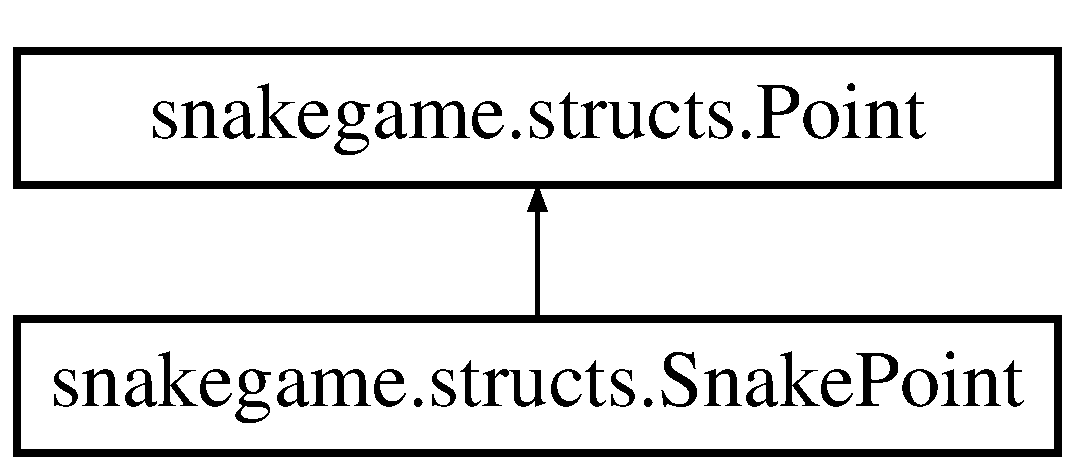
\includegraphics[height=2.000000cm]{classsnakegame_1_1structs_1_1_snake_point}
\end{center}
\end{figure}
\subsection*{Public Member Functions}
\begin{DoxyCompactItemize}
\item 
\mbox{\hyperlink{classsnakegame_1_1structs_1_1_snake_point_ae366301b429df98a08689c778a097d7c}{Snake\+Point}} (\mbox{\hyperlink{classsnakegame_1_1structs_1_1_remainder}{Remainder}} \mbox{\hyperlink{classsnakegame_1_1structs_1_1_point_acf6c91ee7cda0e65a8054ff0dc07b79a}{x}}, \mbox{\hyperlink{classsnakegame_1_1structs_1_1_remainder}{Remainder}} \mbox{\hyperlink{classsnakegame_1_1structs_1_1_point_a2a9fe55d9cf57dbc120bbce39313d38d}{y}})
\item 
void \mbox{\hyperlink{classsnakegame_1_1structs_1_1_snake_point_aa226b89f8a362d365d5f1d1b522aabaf}{draw}} (Graphics2D g)
\end{DoxyCompactItemize}
\subsection*{Additional Inherited Members}


\subsection{Detailed Description}


Definition at line 5 of file Snake\+Point.\+java.



\subsection{Constructor \& Destructor Documentation}
\mbox{\Hypertarget{classsnakegame_1_1structs_1_1_snake_point_ae366301b429df98a08689c778a097d7c}\label{classsnakegame_1_1structs_1_1_snake_point_ae366301b429df98a08689c778a097d7c}} 
\index{snakegame\+::structs\+::\+Snake\+Point@{snakegame\+::structs\+::\+Snake\+Point}!Snake\+Point@{Snake\+Point}}
\index{Snake\+Point@{Snake\+Point}!snakegame\+::structs\+::\+Snake\+Point@{snakegame\+::structs\+::\+Snake\+Point}}
\subsubsection{\texorpdfstring{Snake\+Point()}{SnakePoint()}}
{\footnotesize\ttfamily snakegame.\+structs.\+Snake\+Point.\+Snake\+Point (\begin{DoxyParamCaption}\item[{\mbox{\hyperlink{classsnakegame_1_1structs_1_1_remainder}{Remainder}}}]{x,  }\item[{\mbox{\hyperlink{classsnakegame_1_1structs_1_1_remainder}{Remainder}}}]{y }\end{DoxyParamCaption})}



Definition at line 9 of file Snake\+Point.\+java.



\subsection{Member Function Documentation}
\mbox{\Hypertarget{classsnakegame_1_1structs_1_1_snake_point_aa226b89f8a362d365d5f1d1b522aabaf}\label{classsnakegame_1_1structs_1_1_snake_point_aa226b89f8a362d365d5f1d1b522aabaf}} 
\index{snakegame\+::structs\+::\+Snake\+Point@{snakegame\+::structs\+::\+Snake\+Point}!draw@{draw}}
\index{draw@{draw}!snakegame\+::structs\+::\+Snake\+Point@{snakegame\+::structs\+::\+Snake\+Point}}
\subsubsection{\texorpdfstring{draw()}{draw()}}
{\footnotesize\ttfamily void snakegame.\+structs.\+Snake\+Point.\+draw (\begin{DoxyParamCaption}\item[{Graphics2D}]{g }\end{DoxyParamCaption})}



Definition at line 14 of file Snake\+Point.\+java.



The documentation for this class was generated from the following file\+:\begin{DoxyCompactItemize}
\item 
src/snakegame/structs/\mbox{\hyperlink{_snake_point_8java}{Snake\+Point.\+java}}\end{DoxyCompactItemize}

\hypertarget{classsnakegame_1_1structs_1_1_world}{}\section{snakegame.\+structs.\+World Class Reference}
\label{classsnakegame_1_1structs_1_1_world}\index{snakegame.\+structs.\+World@{snakegame.\+structs.\+World}}
\subsection*{Public Member Functions}
\begin{DoxyCompactItemize}
\item 
\mbox{\hyperlink{classsnakegame_1_1structs_1_1_world_a5ae70562a085bef9fe1f6c718fae1385}{World}} (List$<$ \mbox{\hyperlink{classsnakegame_1_1structs_1_1_apple}{Apple}} $>$ apples, List$<$ \mbox{\hyperlink{classsnakegame_1_1structs_1_1_snake}{Snake}} $>$ snakes)
\item 
void \mbox{\hyperlink{classsnakegame_1_1structs_1_1_world_aa60efdc485c049d8011fb6c50feead00}{process\+Message}} (\mbox{\hyperlink{classsnakegame_1_1server_1_1_message}{Message}} message)
\item 
\mbox{\hyperlink{classsnakegame_1_1structs_1_1_world_ae2e3d1b007bf6a7dc55fb38443719abb}{World}} ()
\item 
void \mbox{\hyperlink{classsnakegame_1_1structs_1_1_world_aca40cde5e48ac321fdf87d207c2b07bc}{draw}} (Graphics2D g)
\item 
void \mbox{\hyperlink{classsnakegame_1_1structs_1_1_world_a0ade5918df8724d3af19bea782932a96}{generate\+Apple}} ()
\item 
U\+U\+ID \mbox{\hyperlink{classsnakegame_1_1structs_1_1_world_a64c7e69961c14046814619a7365f8630}{generate\+Snake}} ()
\item 
void \mbox{\hyperlink{classsnakegame_1_1structs_1_1_world_a3da1e90d5d7e475e900171540123c9e3}{step}} ()
\item 
String \mbox{\hyperlink{classsnakegame_1_1structs_1_1_world_a4b6e33ad84c2ab6d5156acb1d32cdcff}{to\+String}} ()
\end{DoxyCompactItemize}
\subsection*{Static Public Member Functions}
\begin{DoxyCompactItemize}
\item 
static \mbox{\hyperlink{classsnakegame_1_1structs_1_1_world}{World}} \mbox{\hyperlink{classsnakegame_1_1structs_1_1_world_ab8c00c8a748680c55739b31c51d50af5}{parse}} (String string)  throws Illegal\+Argument\+Exception
\end{DoxyCompactItemize}


\subsection{Detailed Description}


Definition at line 11 of file World.\+java.



\subsection{Constructor \& Destructor Documentation}
\mbox{\Hypertarget{classsnakegame_1_1structs_1_1_world_a5ae70562a085bef9fe1f6c718fae1385}\label{classsnakegame_1_1structs_1_1_world_a5ae70562a085bef9fe1f6c718fae1385}} 
\index{snakegame\+::structs\+::\+World@{snakegame\+::structs\+::\+World}!World@{World}}
\index{World@{World}!snakegame\+::structs\+::\+World@{snakegame\+::structs\+::\+World}}
\subsubsection{\texorpdfstring{World()}{World()}\hspace{0.1cm}{\footnotesize\ttfamily [1/2]}}
{\footnotesize\ttfamily snakegame.\+structs.\+World.\+World (\begin{DoxyParamCaption}\item[{List$<$ \mbox{\hyperlink{classsnakegame_1_1structs_1_1_apple}{Apple}} $>$}]{apples,  }\item[{List$<$ \mbox{\hyperlink{classsnakegame_1_1structs_1_1_snake}{Snake}} $>$}]{snakes }\end{DoxyParamCaption})}



Definition at line 18 of file World.\+java.

\mbox{\Hypertarget{classsnakegame_1_1structs_1_1_world_ae2e3d1b007bf6a7dc55fb38443719abb}\label{classsnakegame_1_1structs_1_1_world_ae2e3d1b007bf6a7dc55fb38443719abb}} 
\index{snakegame\+::structs\+::\+World@{snakegame\+::structs\+::\+World}!World@{World}}
\index{World@{World}!snakegame\+::structs\+::\+World@{snakegame\+::structs\+::\+World}}
\subsubsection{\texorpdfstring{World()}{World()}\hspace{0.1cm}{\footnotesize\ttfamily [2/2]}}
{\footnotesize\ttfamily snakegame.\+structs.\+World.\+World (\begin{DoxyParamCaption}{ }\end{DoxyParamCaption})}



Definition at line 33 of file World.\+java.



\subsection{Member Function Documentation}
\mbox{\Hypertarget{classsnakegame_1_1structs_1_1_world_aca40cde5e48ac321fdf87d207c2b07bc}\label{classsnakegame_1_1structs_1_1_world_aca40cde5e48ac321fdf87d207c2b07bc}} 
\index{snakegame\+::structs\+::\+World@{snakegame\+::structs\+::\+World}!draw@{draw}}
\index{draw@{draw}!snakegame\+::structs\+::\+World@{snakegame\+::structs\+::\+World}}
\subsubsection{\texorpdfstring{draw()}{draw()}}
{\footnotesize\ttfamily void snakegame.\+structs.\+World.\+draw (\begin{DoxyParamCaption}\item[{Graphics2D}]{g }\end{DoxyParamCaption})}



Definition at line 39 of file World.\+java.

\mbox{\Hypertarget{classsnakegame_1_1structs_1_1_world_a0ade5918df8724d3af19bea782932a96}\label{classsnakegame_1_1structs_1_1_world_a0ade5918df8724d3af19bea782932a96}} 
\index{snakegame\+::structs\+::\+World@{snakegame\+::structs\+::\+World}!generate\+Apple@{generate\+Apple}}
\index{generate\+Apple@{generate\+Apple}!snakegame\+::structs\+::\+World@{snakegame\+::structs\+::\+World}}
\subsubsection{\texorpdfstring{generate\+Apple()}{generateApple()}}
{\footnotesize\ttfamily void snakegame.\+structs.\+World.\+generate\+Apple (\begin{DoxyParamCaption}{ }\end{DoxyParamCaption})}



Definition at line 50 of file World.\+java.

\mbox{\Hypertarget{classsnakegame_1_1structs_1_1_world_a64c7e69961c14046814619a7365f8630}\label{classsnakegame_1_1structs_1_1_world_a64c7e69961c14046814619a7365f8630}} 
\index{snakegame\+::structs\+::\+World@{snakegame\+::structs\+::\+World}!generate\+Snake@{generate\+Snake}}
\index{generate\+Snake@{generate\+Snake}!snakegame\+::structs\+::\+World@{snakegame\+::structs\+::\+World}}
\subsubsection{\texorpdfstring{generate\+Snake()}{generateSnake()}}
{\footnotesize\ttfamily U\+U\+ID snakegame.\+structs.\+World.\+generate\+Snake (\begin{DoxyParamCaption}{ }\end{DoxyParamCaption})}



Definition at line 55 of file World.\+java.

\mbox{\Hypertarget{classsnakegame_1_1structs_1_1_world_ab8c00c8a748680c55739b31c51d50af5}\label{classsnakegame_1_1structs_1_1_world_ab8c00c8a748680c55739b31c51d50af5}} 
\index{snakegame\+::structs\+::\+World@{snakegame\+::structs\+::\+World}!parse@{parse}}
\index{parse@{parse}!snakegame\+::structs\+::\+World@{snakegame\+::structs\+::\+World}}
\subsubsection{\texorpdfstring{parse()}{parse()}}
{\footnotesize\ttfamily static \mbox{\hyperlink{classsnakegame_1_1structs_1_1_world}{World}} snakegame.\+structs.\+World.\+parse (\begin{DoxyParamCaption}\item[{String}]{string }\end{DoxyParamCaption}) throws Illegal\+Argument\+Exception\hspace{0.3cm}{\ttfamily [static]}}



Definition at line 113 of file World.\+java.

\mbox{\Hypertarget{classsnakegame_1_1structs_1_1_world_aa60efdc485c049d8011fb6c50feead00}\label{classsnakegame_1_1structs_1_1_world_aa60efdc485c049d8011fb6c50feead00}} 
\index{snakegame\+::structs\+::\+World@{snakegame\+::structs\+::\+World}!process\+Message@{process\+Message}}
\index{process\+Message@{process\+Message}!snakegame\+::structs\+::\+World@{snakegame\+::structs\+::\+World}}
\subsubsection{\texorpdfstring{process\+Message()}{processMessage()}}
{\footnotesize\ttfamily void snakegame.\+structs.\+World.\+process\+Message (\begin{DoxyParamCaption}\item[{\mbox{\hyperlink{classsnakegame_1_1server_1_1_message}{Message}}}]{message }\end{DoxyParamCaption})}



Definition at line 24 of file World.\+java.

\mbox{\Hypertarget{classsnakegame_1_1structs_1_1_world_a3da1e90d5d7e475e900171540123c9e3}\label{classsnakegame_1_1structs_1_1_world_a3da1e90d5d7e475e900171540123c9e3}} 
\index{snakegame\+::structs\+::\+World@{snakegame\+::structs\+::\+World}!step@{step}}
\index{step@{step}!snakegame\+::structs\+::\+World@{snakegame\+::structs\+::\+World}}
\subsubsection{\texorpdfstring{step()}{step()}}
{\footnotesize\ttfamily void snakegame.\+structs.\+World.\+step (\begin{DoxyParamCaption}{ }\end{DoxyParamCaption})}



Definition at line 62 of file World.\+java.

\mbox{\Hypertarget{classsnakegame_1_1structs_1_1_world_a4b6e33ad84c2ab6d5156acb1d32cdcff}\label{classsnakegame_1_1structs_1_1_world_a4b6e33ad84c2ab6d5156acb1d32cdcff}} 
\index{snakegame\+::structs\+::\+World@{snakegame\+::structs\+::\+World}!to\+String@{to\+String}}
\index{to\+String@{to\+String}!snakegame\+::structs\+::\+World@{snakegame\+::structs\+::\+World}}
\subsubsection{\texorpdfstring{to\+String()}{toString()}}
{\footnotesize\ttfamily String snakegame.\+structs.\+World.\+to\+String (\begin{DoxyParamCaption}{ }\end{DoxyParamCaption})}



Definition at line 99 of file World.\+java.



The documentation for this class was generated from the following file\+:\begin{DoxyCompactItemize}
\item 
src/snakegame/structs/\mbox{\hyperlink{_world_8java}{World.\+java}}\end{DoxyCompactItemize}

\hypertarget{classsnakegame_1_1server_1_1_server_1_1_world_updater}{}\section{snakegame.\+server.\+Server.\+World\+Updater Class Reference}
\label{classsnakegame_1_1server_1_1_server_1_1_world_updater}\index{snakegame.\+server.\+Server.\+World\+Updater@{snakegame.\+server.\+Server.\+World\+Updater}}
Inheritance diagram for snakegame.\+server.\+Server.\+World\+Updater\+:\begin{figure}[H]
\begin{center}
\leavevmode
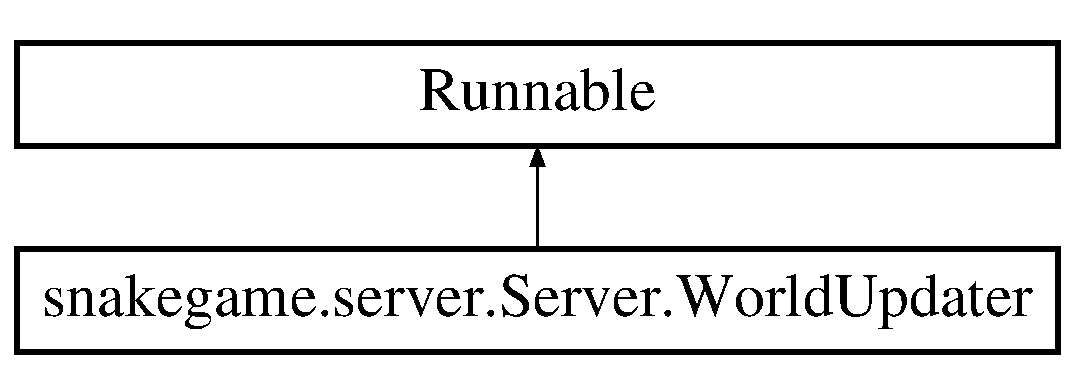
\includegraphics[height=2.000000cm]{classsnakegame_1_1server_1_1_server_1_1_world_updater}
\end{center}
\end{figure}
\subsection*{Public Member Functions}
\begin{DoxyCompactItemize}
\item 
void \mbox{\hyperlink{classsnakegame_1_1server_1_1_server_1_1_world_updater_ab5b9d807315109ef40781908856852dd}{run}} ()
\item 
void \mbox{\hyperlink{classsnakegame_1_1server_1_1_server_1_1_world_updater_ab7308f88031d3de36fe9625235b5cfc3}{process\+Messages}} ()
\end{DoxyCompactItemize}


\subsection{Detailed Description}


Definition at line 161 of file Server.\+java.



\subsection{Member Function Documentation}
\mbox{\Hypertarget{classsnakegame_1_1server_1_1_server_1_1_world_updater_ab7308f88031d3de36fe9625235b5cfc3}\label{classsnakegame_1_1server_1_1_server_1_1_world_updater_ab7308f88031d3de36fe9625235b5cfc3}} 
\index{snakegame\+::server\+::\+Server\+::\+World\+Updater@{snakegame\+::server\+::\+Server\+::\+World\+Updater}!process\+Messages@{process\+Messages}}
\index{process\+Messages@{process\+Messages}!snakegame\+::server\+::\+Server\+::\+World\+Updater@{snakegame\+::server\+::\+Server\+::\+World\+Updater}}
\subsubsection{\texorpdfstring{process\+Messages()}{processMessages()}}
{\footnotesize\ttfamily void snakegame.\+server.\+Server.\+World\+Updater.\+process\+Messages (\begin{DoxyParamCaption}{ }\end{DoxyParamCaption})}



Definition at line 185 of file Server.\+java.

\mbox{\Hypertarget{classsnakegame_1_1server_1_1_server_1_1_world_updater_ab5b9d807315109ef40781908856852dd}\label{classsnakegame_1_1server_1_1_server_1_1_world_updater_ab5b9d807315109ef40781908856852dd}} 
\index{snakegame\+::server\+::\+Server\+::\+World\+Updater@{snakegame\+::server\+::\+Server\+::\+World\+Updater}!run@{run}}
\index{run@{run}!snakegame\+::server\+::\+Server\+::\+World\+Updater@{snakegame\+::server\+::\+Server\+::\+World\+Updater}}
\subsubsection{\texorpdfstring{run()}{run()}}
{\footnotesize\ttfamily void snakegame.\+server.\+Server.\+World\+Updater.\+run (\begin{DoxyParamCaption}{ }\end{DoxyParamCaption})}



Definition at line 163 of file Server.\+java.



The documentation for this class was generated from the following file\+:\begin{DoxyCompactItemize}
\item 
src/snakegame/server/\mbox{\hyperlink{_server_8java}{Server.\+java}}\end{DoxyCompactItemize}

\chapter{File Documentation}
\hypertarget{apple_8java}{}\section{src/snakegame/apple.java File Reference}
\label{apple_8java}\index{src/snakegame/apple.\+java@{src/snakegame/apple.\+java}}
\subsection*{Classes}
\begin{DoxyCompactItemize}
\item 
class \mbox{\hyperlink{classsnakegame_1_1apple}{snakegame.\+apple}}
\end{DoxyCompactItemize}
\subsection*{Packages}
\begin{DoxyCompactItemize}
\item 
package \mbox{\hyperlink{namespacesnakegame}{snakegame}}
\end{DoxyCompactItemize}

\hypertarget{structs_2apple_8java}{}\section{src/snakegame/structs/\+Apple.java File Reference}
\label{structs_2apple_8java}\index{src/snakegame/structs/\+Apple.\+java@{src/snakegame/structs/\+Apple.\+java}}
\subsection*{Classes}
\begin{DoxyCompactItemize}
\item 
class \mbox{\hyperlink{classsnakegame_1_1structs_1_1_apple}{snakegame.\+structs.\+Apple}}
\end{DoxyCompactItemize}
\subsection*{Packages}
\begin{DoxyCompactItemize}
\item 
package \mbox{\hyperlink{namespacesnakegame_1_1structs}{snakegame.\+structs}}
\end{DoxyCompactItemize}

\hypertarget{_client_8java}{}\section{src/snakegame/client/\+Client.java File Reference}
\label{_client_8java}\index{src/snakegame/client/\+Client.\+java@{src/snakegame/client/\+Client.\+java}}
\subsection*{Classes}
\begin{DoxyCompactItemize}
\item 
class \mbox{\hyperlink{classsnakegame_1_1client_1_1_client}{snakegame.\+client.\+Client}}
\item 
class {\bfseries snakegame.\+client.\+Client.\+Client\+Key\+Listener}
\end{DoxyCompactItemize}
\subsection*{Packages}
\begin{DoxyCompactItemize}
\item 
package \mbox{\hyperlink{namespacesnakegame_1_1client}{snakegame.\+client}}
\end{DoxyCompactItemize}

\hypertarget{_constants_8java}{}\section{src/snakegame/\+Constants.java File Reference}
\label{_constants_8java}\index{src/snakegame/\+Constants.\+java@{src/snakegame/\+Constants.\+java}}
\subsection*{Classes}
\begin{DoxyCompactItemize}
\item 
class \mbox{\hyperlink{classsnakegame_1_1_constants}{snakegame.\+Constants}}
\end{DoxyCompactItemize}
\subsection*{Packages}
\begin{DoxyCompactItemize}
\item 
package \mbox{\hyperlink{namespacesnakegame}{snakegame}}
\end{DoxyCompactItemize}

\hypertarget{_game_8java}{}\section{src/snakegame/\+Game.java File Reference}
\label{_game_8java}\index{src/snakegame/\+Game.\+java@{src/snakegame/\+Game.\+java}}
\subsection*{Classes}
\begin{DoxyCompactItemize}
\item 
class \mbox{\hyperlink{classsnakegame_1_1_game}{snakegame.\+Game}}
\end{DoxyCompactItemize}
\subsection*{Packages}
\begin{DoxyCompactItemize}
\item 
package \mbox{\hyperlink{namespacesnakegame}{snakegame}}
\end{DoxyCompactItemize}

\hypertarget{_main_window_8java}{}\section{src/snakegame/\+Main\+Window.java File Reference}
\label{_main_window_8java}\index{src/snakegame/\+Main\+Window.\+java@{src/snakegame/\+Main\+Window.\+java}}
\subsection*{Classes}
\begin{DoxyCompactItemize}
\item 
class \mbox{\hyperlink{classsnakegame_1_1_main_window}{snakegame.\+Main\+Window}}
\end{DoxyCompactItemize}
\subsection*{Packages}
\begin{DoxyCompactItemize}
\item 
package \mbox{\hyperlink{namespacesnakegame}{snakegame}}
\end{DoxyCompactItemize}

\hypertarget{_contriols_queue_8java}{}\section{src/snakegame/server/\+Contriols\+Queue.java File Reference}
\label{_contriols_queue_8java}\index{src/snakegame/server/\+Contriols\+Queue.\+java@{src/snakegame/server/\+Contriols\+Queue.\+java}}
\subsection*{Classes}
\begin{DoxyCompactItemize}
\item 
class \mbox{\hyperlink{classsnakegame_1_1server_1_1_contriols_queue}{snakegame.\+server.\+Contriols\+Queue}}
\end{DoxyCompactItemize}
\subsection*{Packages}
\begin{DoxyCompactItemize}
\item 
package \mbox{\hyperlink{namespacesnakegame_1_1server}{snakegame.\+server}}
\end{DoxyCompactItemize}

\hypertarget{_message_8java}{}\section{src/snakegame/server/\+Message.java File Reference}
\label{_message_8java}\index{src/snakegame/server/\+Message.\+java@{src/snakegame/server/\+Message.\+java}}
\subsection*{Classes}
\begin{DoxyCompactItemize}
\item 
class \mbox{\hyperlink{classsnakegame_1_1server_1_1_message}{snakegame.\+server.\+Message}}
\end{DoxyCompactItemize}
\subsection*{Packages}
\begin{DoxyCompactItemize}
\item 
package \mbox{\hyperlink{namespacesnakegame_1_1server}{snakegame.\+server}}
\end{DoxyCompactItemize}

\hypertarget{_server_8java}{}\section{src/snakegame/server/\+Server.java File Reference}
\label{_server_8java}\index{src/snakegame/server/\+Server.\+java@{src/snakegame/server/\+Server.\+java}}
\subsection*{Classes}
\begin{DoxyCompactItemize}
\item 
class \mbox{\hyperlink{classsnakegame_1_1server_1_1_server}{snakegame.\+server.\+Server}}
\item 
class \mbox{\hyperlink{classsnakegame_1_1server_1_1_server_1_1_client_handler}{snakegame.\+server.\+Server.\+Client\+Handler}}
\item 
class \mbox{\hyperlink{classsnakegame_1_1server_1_1_server_1_1_client_updater}{snakegame.\+server.\+Server.\+Client\+Updater}}
\item 
class \mbox{\hyperlink{classsnakegame_1_1server_1_1_server_1_1_world_updater}{snakegame.\+server.\+Server.\+World\+Updater}}
\end{DoxyCompactItemize}
\subsection*{Packages}
\begin{DoxyCompactItemize}
\item 
package \mbox{\hyperlink{namespacesnakegame_1_1server}{snakegame.\+server}}
\end{DoxyCompactItemize}

\hypertarget{snake_8java}{}\section{src/snakegame/snake.java File Reference}
\label{snake_8java}\index{src/snakegame/snake.\+java@{src/snakegame/snake.\+java}}
\subsection*{Classes}
\begin{DoxyCompactItemize}
\item 
class \mbox{\hyperlink{classsnakegame_1_1snake}{snakegame.\+snake}}
\end{DoxyCompactItemize}
\subsection*{Packages}
\begin{DoxyCompactItemize}
\item 
package \mbox{\hyperlink{namespacesnakegame}{snakegame}}
\end{DoxyCompactItemize}

\hypertarget{structs_2snake_8java}{}\section{src/snakegame/structs/\+Snake.java File Reference}
\label{structs_2snake_8java}\index{src/snakegame/structs/\+Snake.\+java@{src/snakegame/structs/\+Snake.\+java}}
\subsection*{Classes}
\begin{DoxyCompactItemize}
\item 
class \mbox{\hyperlink{classsnakegame_1_1structs_1_1_snake}{snakegame.\+structs.\+Snake}}
\end{DoxyCompactItemize}
\subsection*{Packages}
\begin{DoxyCompactItemize}
\item 
package \mbox{\hyperlink{namespacesnakegame_1_1structs}{snakegame.\+structs}}
\end{DoxyCompactItemize}

\hypertarget{_apple_factory_8java}{}\section{src/snakegame/structs/\+Apple\+Factory.java File Reference}
\label{_apple_factory_8java}\index{src/snakegame/structs/\+Apple\+Factory.\+java@{src/snakegame/structs/\+Apple\+Factory.\+java}}
\subsection*{Classes}
\begin{DoxyCompactItemize}
\item 
class \mbox{\hyperlink{classsnakegame_1_1structs_1_1_apple_factory}{snakegame.\+structs.\+Apple\+Factory}}
\end{DoxyCompactItemize}
\subsection*{Packages}
\begin{DoxyCompactItemize}
\item 
package \mbox{\hyperlink{namespacesnakegame_1_1structs}{snakegame.\+structs}}
\end{DoxyCompactItemize}

\hypertarget{_apple_point_8java}{}\section{src/snakegame/structs/\+Apple\+Point.java File Reference}
\label{_apple_point_8java}\index{src/snakegame/structs/\+Apple\+Point.\+java@{src/snakegame/structs/\+Apple\+Point.\+java}}
\subsection*{Classes}
\begin{DoxyCompactItemize}
\item 
class \mbox{\hyperlink{classsnakegame_1_1structs_1_1_apple_point}{snakegame.\+structs.\+Apple\+Point}}
\end{DoxyCompactItemize}
\subsection*{Packages}
\begin{DoxyCompactItemize}
\item 
package \mbox{\hyperlink{namespacesnakegame_1_1structs}{snakegame.\+structs}}
\end{DoxyCompactItemize}

\hypertarget{_direction_8java}{}\section{src/snakegame/structs/\+Direction.java File Reference}
\label{_direction_8java}\index{src/snakegame/structs/\+Direction.\+java@{src/snakegame/structs/\+Direction.\+java}}
\subsection*{Classes}
\begin{DoxyCompactItemize}
\item 
enum \mbox{\hyperlink{enumsnakegame_1_1structs_1_1_direction}{snakegame.\+structs.\+Direction}}
\end{DoxyCompactItemize}
\subsection*{Packages}
\begin{DoxyCompactItemize}
\item 
package \mbox{\hyperlink{namespacesnakegame_1_1structs}{snakegame.\+structs}}
\end{DoxyCompactItemize}

\hypertarget{_point_8java}{}\section{src/snakegame/structs/\+Point.java File Reference}
\label{_point_8java}\index{src/snakegame/structs/\+Point.\+java@{src/snakegame/structs/\+Point.\+java}}
\subsection*{Classes}
\begin{DoxyCompactItemize}
\item 
class \mbox{\hyperlink{classsnakegame_1_1structs_1_1_point}{snakegame.\+structs.\+Point}}
\end{DoxyCompactItemize}
\subsection*{Packages}
\begin{DoxyCompactItemize}
\item 
package \mbox{\hyperlink{namespacesnakegame_1_1structs}{snakegame.\+structs}}
\end{DoxyCompactItemize}

\hypertarget{_remainder_8java}{}\section{src/snakegame/structs/\+Remainder.java File Reference}
\label{_remainder_8java}\index{src/snakegame/structs/\+Remainder.\+java@{src/snakegame/structs/\+Remainder.\+java}}
\subsection*{Classes}
\begin{DoxyCompactItemize}
\item 
class \mbox{\hyperlink{classsnakegame_1_1structs_1_1_remainder}{snakegame.\+structs.\+Remainder}}
\end{DoxyCompactItemize}
\subsection*{Packages}
\begin{DoxyCompactItemize}
\item 
package \mbox{\hyperlink{namespacesnakegame_1_1structs}{snakegame.\+structs}}
\end{DoxyCompactItemize}

\hypertarget{_snake_factory_8java}{}\section{src/snakegame/structs/\+Snake\+Factory.java File Reference}
\label{_snake_factory_8java}\index{src/snakegame/structs/\+Snake\+Factory.\+java@{src/snakegame/structs/\+Snake\+Factory.\+java}}
\subsection*{Classes}
\begin{DoxyCompactItemize}
\item 
class \mbox{\hyperlink{classsnakegame_1_1structs_1_1_snake_factory}{snakegame.\+structs.\+Snake\+Factory}}
\end{DoxyCompactItemize}
\subsection*{Packages}
\begin{DoxyCompactItemize}
\item 
package \mbox{\hyperlink{namespacesnakegame_1_1structs}{snakegame.\+structs}}
\end{DoxyCompactItemize}

\hypertarget{_snake_point_8java}{}\section{src/snakegame/structs/\+Snake\+Point.java File Reference}
\label{_snake_point_8java}\index{src/snakegame/structs/\+Snake\+Point.\+java@{src/snakegame/structs/\+Snake\+Point.\+java}}
\subsection*{Classes}
\begin{DoxyCompactItemize}
\item 
class \mbox{\hyperlink{classsnakegame_1_1structs_1_1_snake_point}{snakegame.\+structs.\+Snake\+Point}}
\end{DoxyCompactItemize}
\subsection*{Packages}
\begin{DoxyCompactItemize}
\item 
package \mbox{\hyperlink{namespacesnakegame_1_1structs}{snakegame.\+structs}}
\end{DoxyCompactItemize}

\hypertarget{_world_8java}{}\section{src/snakegame/structs/\+World.java File Reference}
\label{_world_8java}\index{src/snakegame/structs/\+World.\+java@{src/snakegame/structs/\+World.\+java}}
\subsection*{Classes}
\begin{DoxyCompactItemize}
\item 
class \mbox{\hyperlink{classsnakegame_1_1structs_1_1_world}{snakegame.\+structs.\+World}}
\end{DoxyCompactItemize}
\subsection*{Packages}
\begin{DoxyCompactItemize}
\item 
package \mbox{\hyperlink{namespacesnakegame_1_1structs}{snakegame.\+structs}}
\end{DoxyCompactItemize}

%--- End generated contents ---

% Index
\backmatter
\newpage
\phantomsection
\clearemptydoublepage
\addcontentsline{toc}{chapter}{Index}
\printindex

\end{document}
